%\documentclass[12pt,vi,twoside]{mitthesis}
%%
%%  If you want your thesis copyright to you instead of MIT, use the
%%  ``vi'' option, as above.
%%
%\documentclass[12pt,twoside,leftblank]{mitthesis}
%%
%% If you want blank pages before new chapters to be labelled ``This
%% Page Intentionally Left Blank'', use the ``leftblank'' option, as
%% above. 

\documentclass[12pt,oneside]{SETUP/mitthesis}
\pagestyle{plain}
\usepackage{SETUP/lgrind}
\usepackage{cmap}
\usepackage[T1]{fontenc}
\usepackage[colorlinks=true,linkcolor=blue]{hyperref}
\usepackage[svgnames]{xcolor}
\hypersetup{colorlinks,breaklinks,
      linkcolor = NavyBlue,
      urlcolor  = NavyBlue,
      citecolor = NavyBlue,
      anchorcolor = NavyBlue,
      linkcolor = NavyBlue
}
\usepackage{epsfig}
\usepackage{graphicx}
\usepackage{grffile}
\usepackage{epstopdf}
\usepackage{amsmath,amssymb,amsfonts,latexsym}
\usepackage{placeins}
% \usepackage{bbm,vector}
\usepackage{enumitem}
%\usepackage[english, algoruled, noline, norelsize]{algorithm2e}
\usepackage[english, algoruled, noline]{algorithm2e}
\usepackage{url}	
\usepackage[caption=false]{subfig}
\usepackage[titletoc]{appendix}
\usepackage{expl3}

%%My definitions
\ExplSyntaxOn
\newcommand\latinabbrev[1]{
  \peek_meaning:NTF . {% Same as \@ifnextchar
    #1\@}%
  { \peek_catcode:NTF a {% Check whether next char has same catcode as \'a, i.e., is a letter
      #1.\@ }%
    {#1.\@}}}
\ExplSyntaxOff

%Omit final dot from each def.
\def\eg{\latinabbrev{e.g}}
\def\etal{\latinabbrev{et al}}
\def\etc{\latinabbrev{etc}}
\def\ie{\latinabbrev{i.e}}

\DeclareGraphicsExtensions{.pdf,.png,.jpg}

%For frame
\def\W{\mathcal{W}} 
\def\I{\mathcal{I}}
\def\C{\mathcal{C}}
\def\F{\mathcal{F}}
\def\A{\mathcal{A}}
\def\B{\mathcal{B}}
\def\C{\mathcal{C}}

%For matrix
\def\mA{\mathbf{A}}
\def\mB{\mathbf{B}}
\def\mC{\mathbf{C}}
\def\mR{\mathbf{R}}
\def\mSigma{\mathbf{\Sigma}}
\def\mJ{\mathbf{J}}
\def\mW{\mathbf{W}}
\def\mK{\mathbf{K}}
\def\mH{\mathbf{H}}
\def\mI{\mathbf{I}}

\renewcommand{\vec}[1]{\boldsymbol{#1}}
\newcommand{\norm}[1]{\left\|#1\right\|}

\def\ones{\mathbf{1}}

\def\argmin{\mathop{\rm arg\,min}\limits}

\usepackage{array}
\newcolumntype{P}[1]{>{\centering\arraybackslash}p{#1}}
\newcolumntype{M}[1]{>{\centering\arraybackslash}m{#1}}
%%My definitions end

\begin{document}
  
\title{Keyframe-based Visual-Inertial Odometry for Small Workspace}
\author{Xi Li}

% You can use the \\ command to list multiple previous degrees
%       \prevdegrees{B.S., University of California (1978) \\
%                    S.M., Massachusetts Institute of Technology (1981)}
\department{Department of Computer Science}

% If the thesis is for two degrees simultaneously, list them both
% separated by \and like this:
% \degree{Doctor of Philosophy \and Master of Science}
\degree{Master of Science in Computer Science}

% As of the 2007-08 academic year, valid degree months are September, 
% February, or June.  The default is June.
\degreemonth{June}
\degreeyear{2016}
\thesisdate{June 1, 2016}

%% By default, the thesis will be copyrighted to SAAR.  If you need to copyright
%% the thesis to yourself, just specify the `vi' documentclass option.  If for
%% some reason you want to exactly specify the copyright notice text, you can
%% use the \copyrightnoticetext command.  
% \copyrightnoticetext{\copyright Quynh Nguyen Ngoc. All rights reserved.}

% If there is more than one supervisor, use the \supervisor command
% once for each.
\supervisor{Roland Angst}{Dr.}

% This is the department committee chairman, not the thesis committee
% chairman.  You should replace this with your Department's Committee
% Chairman.
\chairman{Prof}{Chairman, Department Committee on Graduate Theses}

% Make the titlepage based on the above information.  If you need
% something special and can't use the standard form, you can specify
% the exact text of the titlepage yourself.  Put it in a titlepage
% environment and leave blank lines where you want vertical space.
% The spaces will be adjusted to fill the entire page.  The dotted
% lines for the signatures are made with the \signature command.

% \maketitle
\noindent
\begin{titlepage}

\includegraphics[width=4cm,natwidth=520,natheight=210]{logo_saarland.png}
\hfill
\begin{minipage}{8cm}
\centering
\vspace{-1.5cm} 
\textbf{Universit\"at des Saarlandes \\ Max-Planck-Institut f\"ur Informatik}
\end{minipage}
\hfill

\includegraphics[width=2.8cm,natwidth=300,natheight=244]{mpg.png}
\vfill

\Large
\textbf{Keyframe-based Visual-Inertial Odometry for Small Workspace}
\vfill

\large
Masterarbeit im Fach Informatik \\
Master's Thesis in Computer Science \\
von / by \\
\textbf{Xi Li} \\
\vfill

angefertigt unter der Leitung von / supervised by \\
\large{\textsc{Dr. Roland Angst}}\\
\vfill

betreut von / advised by \\
\large{\textsc{Dr. Roland Angst}} \\
\vfill

begutachtet von / reviewers \\
\large{\textsc{Dr. Roland Angst \\ Prof. Dr. Antonio Kr{\"u}ger}} \\
\vfill

Saarbr\"ucken, June 2016
\end{titlepage}


% The abstractpage environment sets up everything on the page except
% the text itself.  The title and other header material are put at the
% top of the page, and the supervisors are listed at the bottom.  A
% new page is begun both before and after.  Of course, an abstract may
% be more than one page itself.  If you need more control over the
% format of the page, you can use the abstract environment, which puts
% the word "Abstract" at the beginning and single spaces its text.

%% You can either \input (*not* \include) your abstract file, or you can put
%% the text of the abstract directly between the \begin{abstractpage} and
%% \end{abstractpage} commands.

% First copy: start a new page, and save the page number.
\cleardoublepage
% Uncomment the next line if you do NOT want a page number on your
% abstract and acknowledgments pages.
% \pagestyle{empty}
% \setcounter{savepage}{\thepage}
% \begin{abstractpage}
%     %% The text of your abstract and nothing else (other than comments) goes here.
%% It will be single-spaced and the rest of the text that is supposed to go on
%% the abstract page will be generated by the abstractpage environment.  This
%% file should be \input (not \include 'd) from cover.tex.

Mobile robot navigation has been an attractive topic in the Robotics area for a long time. \textit{Visual SLAM} simultaneously locates robots' poses and constructs a map via analysing measurements obtained from visual sensors. However due to the costly computational complexity of camera, it is non-trivial to gain a high-quality pose estimation while the whole system runs in real-time. \textit{Inertial Measurement Unit} (IMU) measures the rotational rate and acceleration of the robot under the higher output frequency, and it has been considered as an appropriate compensation to a single camera in such navigation systems. In this master thesis, we aim to exploit a visual-inertial odometry, to further improve localization results by fusing visual data and IMU data. More precisely, we apply a loosely-coupled visual-inertial integration method to keep our system runs in a constant time. 

We first discuss the types of visual SLAM. Generally, visual SLAM has two traditional approaches, which are filter-based methods and keyframe-based methods respectively. Filter-based methods marginalise all the previous camera poses to obtain the current pose estimation as well as optimized landmarks, whereas keyframe-based methods keep some of former poses and applies bundle adjustment to further improve the estimation results. We finally choose keyframe-based visual SLAM to be correction data in our Kalman filter framework because it is more efficient when scale of scene becomes larger, another reason is that it can handle loop closures more easily. We then discuss the way to integrate IMU data. We first learn \textit{quaternion} and its operations. Instead of using Euler angle (Gimbal Lock) or rotational matrix (high memory cost), we formulate the system rotation parameters with quaternion. Followed by that, we explain the time-integration and differentiations related to the quaternions, and we suggest a error-state Kalman filter to propagate system states while tracking the system uncertainties. In order to fuse the visual data and IMU data, we suggest an adapted map scale method to automatically propagate the map scale factor, therefore solve the unknown map scale problem existed in mono visual SLAM. A keyframe-based bundle adjustment is then exploited for improving the tracking quality. Our experiments show that our suggested framework obtain more accurate and stable results compared to the state-of-art visual odometry, and our system can be easily extended to large scaled scene.

In addition to Kalman filter based framework, we briefly introduce a manifold optimization approach to solve visual-inertial odometry problem. We have suggested a standard way to solve manifold optimization as well as several ideas to reduce the computational time in the end.


% \end{abstractpage}

% Additional copy: start a new page, and reset the page number.  This way,
% the second copy of the abstract is not counted as separate pages.
% Uncomment the next 6 lines if you need two copies of the abstract
% page.
% \setcounter{page}{\thesavepage}
% \begin{abstractpage}
% %% The text of your abstract and nothing else (other than comments) goes here.
%% It will be single-spaced and the rest of the text that is supposed to go on
%% the abstract page will be generated by the abstractpage environment.  This
%% file should be \input (not \include 'd) from cover.tex.

Mobile robot navigation has been an attractive topic in the Robotics area for a long time. \textit{Visual SLAM} simultaneously locates robots' poses and constructs a map via analysing measurements obtained from visual sensors. However due to the costly computational complexity of camera, it is non-trivial to gain a high-quality pose estimation while the whole system runs in real-time. \textit{Inertial Measurement Unit} (IMU) measures the rotational rate and acceleration of the robot under the higher output frequency, and it has been considered as an appropriate compensation to a single camera in such navigation systems. In this master thesis, we aim to exploit a visual-inertial odometry, to further improve localization results by fusing visual data and IMU data. More precisely, we apply a loosely-coupled visual-inertial integration method to keep our system runs in a constant time. 

We first discuss the types of visual SLAM. Generally, visual SLAM has two traditional approaches, which are filter-based methods and keyframe-based methods respectively. Filter-based methods marginalise all the previous camera poses to obtain the current pose estimation as well as optimized landmarks, whereas keyframe-based methods keep some of former poses and applies bundle adjustment to further improve the estimation results. We finally choose keyframe-based visual SLAM to be correction data in our Kalman filter framework because it is more efficient when scale of scene becomes larger, another reason is that it can handle loop closures more easily. We then discuss the way to integrate IMU data. We first learn \textit{quaternion} and its operations. Instead of using Euler angle (Gimbal Lock) or rotational matrix (high memory cost), we formulate the system rotation parameters with quaternion. Followed by that, we explain the time-integration and differentiations related to the quaternions, and we suggest a error-state Kalman filter to propagate system states while tracking the system uncertainties. In order to fuse the visual data and IMU data, we suggest an adapted map scale method to automatically propagate the map scale factor, therefore solve the unknown map scale problem existed in mono visual SLAM. A keyframe-based bundle adjustment is then exploited for improving the tracking quality. Our experiments show that our suggested framework obtain more accurate and stable results compared to the state-of-art visual odometry, and our system can be easily extended to large scaled scene.

In addition to Kalman filter based framework, we briefly introduce a manifold optimization approach to solve visual-inertial odometry problem. We have suggested a standard way to solve manifold optimization as well as several ideas to reduce the computational time in the end.


% \end{abstractpage}

\cleardoublepage
\pagestyle{empty}
\setcounter{savepage}{\thepage}
\subsubsection*{Eidesstattliche Erkl{\"a}rung}
Ich erkl{\"a}re hiermit an Eides Statt, dass ich die vorliegende Arbeit selbstst{\"a}ndig verfasst und
keine anderen als die angegebenen Quellen und Hilfsmittel verwendet habe.
\subsubsection*{Statement in Lieu of an Oath}
I hereby confirm under oath that I have written this thesis on my own and that I have not
used any other media or materials than the ones referred to in this thesis.

\vspace{1cm}

\subsubsection*{Eidesstattliche Erkl{\"a}rung}
Ich erkl{\"a}re hiermit an Eides Statt, dass die vorliegende Arbeit mit der elektronischen Version {\"u}bereinstimmt.
\subsubsection*{Statement in Lieu of an Oath}
I hereby confirm the congruence of the contents of the printed data and the electronic version of the thesis.

\vspace{1cm}

\subsubsection*{Einverst{\"a}ndniserkl{\"a}rung}
Ich bin damit einverstanden, dass meine (bestandene) Arbeit in beiden Versionen in die
Bibliothek der Informatik aufgenommen und damit ver{\"o}ffentlicht wird.

\subsubsection*{Declaration of Consent}
I agree to make both versions of my thesis (with a passing grade) accessible to the public 
by having them added to the library of the Computer Science Department.

\vspace{3cm}

\par\noindent\makebox[2in]{\hrulefill} 		\hfill\makebox[2in]{\hrulefill}%
\par\noindent\makebox[2in][l]{(Datum / Date)}	\hfill\makebox[2in][l]{(Unterschrift / Signature)}%

\newpage
\section*{Acknowledgments}
I would like to thank Dr. Roland Angst who has been a great supervisor during my thesis. Thanks Dr. Angst for giving me many valuable advise, also keeping a perfect balance of guidance and freedom. 

Also many thanks to members in our group: Dushyant and Rui, who has helped and encouraged me a lot. Special thanks to Rui, Han and Jianan, who has suggested a lot of amazing ideas and helped me to debug my code. Thanks Siwen, Hang for being the proof readers of my master thesis. 

At last I want to thank my parents, who has always give their unconditional supports and love to me. Without their supports and love, I never would have made it.

\pagestyle{empty}
\setcounter{savepage}{\thepage}
\begin{abstractpage}
    %% The text of your abstract and nothing else (other than comments) goes here.
%% It will be single-spaced and the rest of the text that is supposed to go on
%% the abstract page will be generated by the abstractpage environment.  This
%% file should be \input (not \include 'd) from cover.tex.

Mobile robot navigation has been an attractive topic in the Robotics area for a long time. \textit{Visual SLAM} simultaneously locates robots' poses and constructs a map via analysing measurements obtained from visual sensors. However due to the costly computational complexity of camera, it is non-trivial to gain a high-quality pose estimation while the whole system runs in real-time. \textit{Inertial Measurement Unit} (IMU) measures the rotational rate and acceleration of the robot under the higher output frequency, and it has been considered as an appropriate compensation to a single camera in such navigation systems. In this master thesis, we aim to exploit a visual-inertial odometry, to further improve localization results by fusing visual data and IMU data. More precisely, we apply a loosely-coupled visual-inertial integration method to keep our system runs in a constant time. 

We first discuss the types of visual SLAM. Generally, visual SLAM has two traditional approaches, which are filter-based methods and keyframe-based methods respectively. Filter-based methods marginalise all the previous camera poses to obtain the current pose estimation as well as optimized landmarks, whereas keyframe-based methods keep some of former poses and applies bundle adjustment to further improve the estimation results. We finally choose keyframe-based visual SLAM to be correction data in our Kalman filter framework because it is more efficient when scale of scene becomes larger, another reason is that it can handle loop closures more easily. We then discuss the way to integrate IMU data. We first learn \textit{quaternion} and its operations. Instead of using Euler angle (Gimbal Lock) or rotational matrix (high memory cost), we formulate the system rotation parameters with quaternion. Followed by that, we explain the time-integration and differentiations related to the quaternions, and we suggest a error-state Kalman filter to propagate system states while tracking the system uncertainties. In order to fuse the visual data and IMU data, we suggest an adapted map scale method to automatically propagate the map scale factor, therefore solve the unknown map scale problem existed in mono visual SLAM. A keyframe-based bundle adjustment is then exploited for improving the tracking quality. Our experiments show that our suggested framework obtain more accurate and stable results compared to the state-of-art visual odometry, and our system can be easily extended to large scaled scene.

In addition to Kalman filter based framework, we briefly introduce a manifold optimization approach to solve visual-inertial odometry problem. We have suggested a standard way to solve manifold optimization as well as several ideas to reduce the computational time in the end.


\end{abstractpage}

%%%%%%%%%%%%%%%%%%%%%%%%%%%%%%%%%%%%%%%%%%%%%%%%%%%%%%%%%%%%%%%%%%%%%%
% -*-latex-*-

\include{signature}
\pagestyle{plain}
\mbox{}
\thispagestyle{empty}
\newpage
  % -*- Mode:TeX -*-
%% This file simply contains the commands that actually generate the table of
%% contents and lists of figures and tables.  You can omit any or all of
%% these files by simply taking out the appropriate command.  For more
%% information on these files, see appendix C.3.3 of the LaTeX manual. 
\tableofcontents
% \newpage
% \listoffigures
% \newpage
% \listoftables

%% This is an example first chapter.  You should put chapter/appendix that you
%% write into a separate file, and add a line \include{yourfilename} to
%% main.tex, where `yourfilename.tex' is the name of the chapter/appendix file.
%% You can process specific files by typing their names in at the 
%% \files=
%% prompt when you run the file main.tex through LaTeX.
\chapter{Introduction}
\label{chap:intro}

In past few years, the development of \textit{Robotics} has surpassed people's
expectation. The word \textit{Robotics} has been first appeared in science 
fiction "Liar!" by Issac Asimov~\cite{wiki:Robotics}, it referred to science 
and technology of robots. By definition, \textit{Robotics}
is a research branch that related to design, control and application of robots,
as well as processing feedback from robots. 

Modern robots have been classified into several categories(\eg, Mobile robot, 
industrial robot, service robot, education robot \etc) with their usages.
Among those categories, full-autonomous or semi-autonomous mobile robots 
attracts more and more researches. Such robots have  
abilities to move around in their moving space, with or without humans' control.
The aim of research in mobile robots
is to help us accomplish various hard tasks, whether domestically, commercially
or militarily. These tasks, such as assisting disabled people, defusing bombs,
or repair equipment in dangerous place is either risky or high expense for 
human beings.    

For mobile robot, finding physical location of itself in unknown environment 
is normally crucial, 
such an ability(\eg, \textit{Robot Navigation}) allows mobile robots
avoid risky obstacles and finally arrive the goal position. 
Roughly speaking, \textit{Robot Navigation} is a computing system which 
processes the information from external sources(\eg, sensors) and apply an 
algorithm to navigate robot, and sometimes build a map of environment. 
In \textit{Robot Navigation}, robots sense environmental information
by their sensors. These sensors, either locally (\eg, camera, inertial
measurement unit (IMU)), or globally (\eg, Global Positioning System) detect
events or changes in environment, and transfer their data to robots.
Generally, sensors equipped in mobile robot (Local Sensor) are designed light,
small, and inexpensive considering convenient movement and low expense. Camera
and IMU sensor are considered most common local sensor in small mobile robot 
system.

A camera is a optical instrument for capturing images.
Modern camera has several advantages for \textit{Robot Navigation}. First, the
core of camera chip set is cheap
and easily installed in any mobile robot system; Second, camera often brings
very rich information as it simulates the functioning of human eye. By 
recognizing key-points ~\cite{shi1994good, lowe1999object, rosten2010faster}
in certain images, system observes the \textit{landmarks} in environment, and
those \textit{landmarks} will localize robots by \textit{Triangulation}
~\cite{davison2003real, klein2007parallel, eade2007monocular}.

A IMU sensor (Figure~\ref{fig:fig1-1}) often combines \textit{gyroscope} and
\textit{accelerometer}, sometimes \textit{magnetometer}, to measure specific
force, angular rate and magnetic field regarding to its local frame. IMU is
one of main component in \textit{Inertial Navigation System}, which firstly
used in air plane, spacecraft, guided missiles, and now also in mobile robot
~\cite{batalin2004mobile, lee2009position, mourikis2007multi, forster2015imu}.
IMU sensor utilize \textit{Dead Reckoning} to track device's position, such 
technology tries to integrate IMU data over time by assuming the movement 
model of devices fixed(\ie, acceleration and rotation rate is constant over
small period of time). 

\begin{figure}
    \centering
    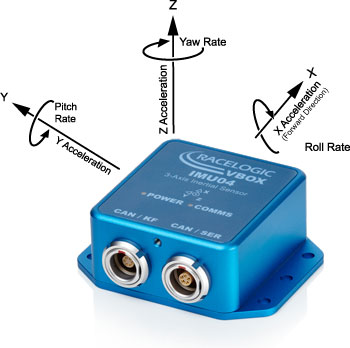
\includegraphics[width=1.0\textwidth]{CONTENT/Figure/Figure1-1_IMU_Sensor.jpg}
    \caption{IMU sensor with gyroscope and accelerometer measures rotational rate
    and acceleration of X, Y, Z axis regarding its local frame. Note that IMU sensor
    normally has bias and irreducible noises, it is necessary to apply a calibration
    like cameras. The frequency of IMU output is normally larger than 100 Hz.
    Source: \cite{Figure1-1_IMU_Sensor}}
    \label{fig:fig1-1}
\end{figure}


\section{Motivation and Contribution}
\label{sec:motiv_contrib}

The main motivation of this thesis is to improve the navigation accuracy by 
fusing camera data and IMU sensor data. 

Single sensor-based navigation
system may not satisfy the requirements of high-quality localization by 
mobile robot.
GPS-based navigation system has been used for outdoor devices for long time.
However, such a system suffered from localizing in in-door environment, and 
also the accuracy of general GPS is not high, \ie, 3 to 5 meters error
\cite{wiki:GPS}. For mobile robot, which may move from in-door to out-door, and
requires high-accuracy navigation, GPS is mostly not used, or as baseline
of navigation~\cite{hesch2014consistency}.   

Vision-based navigation system
\cite{davison2003real, klein2007parallel}, or simultaneous localization and 
mapping (SLAM)~\cite{davison2007monoslam, engel2014lsd, mur2015orb} gives 
an acceptable navigation result. \cite{davison2003real} recognizes corner
feature by single camera, and it uses a extended kalman filter framework to track 
the uncertainty and propagates the system state, however it can not handle
large-scale scene. \cite{klein2007parallel} utilizes key-frame based
bundle adjustment to update the map, improves both accuracy and efficiency,
it still met some problem in large-scale scene, becasue
vision-based method often is
a trade-off between computational complexity and localization accuracy 
due to the rich information and low output frequency by camera. 

Single \textit{Inertial Navigation System} recognize its pose by 
\textit{Dead Reckoning}~\cite{mcnaughton1991dead, levi1996dead}. 
However, the problem of \textit{Dead Reckoning} error
accumulation; Only few directions are observable~\cite{hesch2014consistency}
by IMU during whole navigation process. When object corrupts movement 
assumption, a correction step by external data will be needed.

Fusing camera and IMU data has many advantages. On the one hand,
it can decrease computational time by making good use of high-frequency
IMU data; On the other hand, it can reduce the error accumulation of IMU
integration by the correction of vision-based navigation result within
several turn. Fuse the camera and IMU data for robot navigation is not novel. 
\cite{mourikis2007multi} applies multi-state kalman filter (MSCKF)
on state
update, decrease the computational complexity by only keeping few
last information of keyframe. \cite{hesch2014consistency} analysis
the consistency of MSCKF, correct the ways of IMU integration to 
obtain consistency of sytem, therefore increase the accuracy.
\cite{forster2015imu} exploits a way to optimize manifold information,
therefore solving data fusing problem in a non-linear optimization
scheme. Unfortunately, codes and data of above methods are not 
accessible, that motivates to explore possible methods to increase
accuracy of \textit{vision-inertial navigation system} both theoretically
and experimentally.


The contributions of this thesis are as follows,
\begin{itemize}
\item {We exploit a highly flexible, realistic software to generate
synthetic IMU sensor data and corresponding vision data, that is the
main source to provide experimental data in this thesis.}
\item {We present error-state kalman filter 
system kinematic based on quaternion, explore the 
multiple ways to integrate IMU data due to different movement models.}
\item {We propose a novel method to update fusing result based on 
key-framed bundle adjustment.}
\item {We propose a real-time visual-inertial framework implemented 
in C\texttt{++}, which is stable, scalable, high-accuracy and low-latency.}
\end{itemize}



\section{Outline of the Thesis}
\label{sec:outline}

In Chapter \ref{chap:Overview} we first overview our visual-inertial odometry,
including world representation, important notations, we also compare 
filter method and key-frame based method in SLAM problem, and in the end
we explain our choice in this thesis.

Then we enter the Chapter \ref{chap:background}, which introduces 
\textit{Quaternion Algebra}. In this chapter, we introduces the basic 
operations on quaternion, the relationship among 
quaternion, rotation matrix and rotation vector.
In this chapter, we also explain how to integrate or derivative 
quaternion over time.

Chapter \ref{chap:sensor_fusing} is main part of this thesis. In Section 
\ref{sec:ESKF_IMU},
we study the Error-State Kalman Filter (ESKF), and apply it to IMU integration; 
Section \ref{sec:camera_comple_data} we summarize how to fuse camera into
ESKF, and how to optimize it by key-frame based bundle adjustment. In Section 
\ref{sec:pipeline_overview}, we overview the pipeline of our visual-inertial
odometry system.

We show our experiment results in Chapter \ref{chap:experiments}.
First, the process of generating synthetic IMU and camera data is
presented. Then we run several experiments to show
our proposed visual-inertial odometry has higher accuracy
than  single IMU integration, visual SLAM, as our system is still 
running in real-time.

In the end, we summarize and discuss our work and analysis the potential future work
in Chapter \ref{chap:summary}.

%% This is an example first chapter.  You should put chapter/appendix that you
%% write into a separate file, and add a line \include{yourfilename} to
%% main.tex, where `yourfilename.tex' is the name of the chapter/appendix file.
%% You can process specific files by typing their names in at the 
%% \files=
%% prompt when you run the file main.tex through LaTeX.
\chapter{Overview of Visual-inertial Odometry}
\label{chap:Overview}

In this chapter, we will overview our visual-inertial odometry system. In section \ref{sec:notations}, we first introduce world representation(\eg, world frame, camera frame and IMU frame) together with basic notations in our odometry system. In section \ref{sec:FVK}, we then discuss two important schemes, filter method and keyframe Bundle Adjustment(keyframe BA) in SLAM algorithm, and explain why we finally choose the keyframe-based method.

\section{World Representations and Notations}
\label{sec:notations}

\begin{figure}[h]
    \centering
    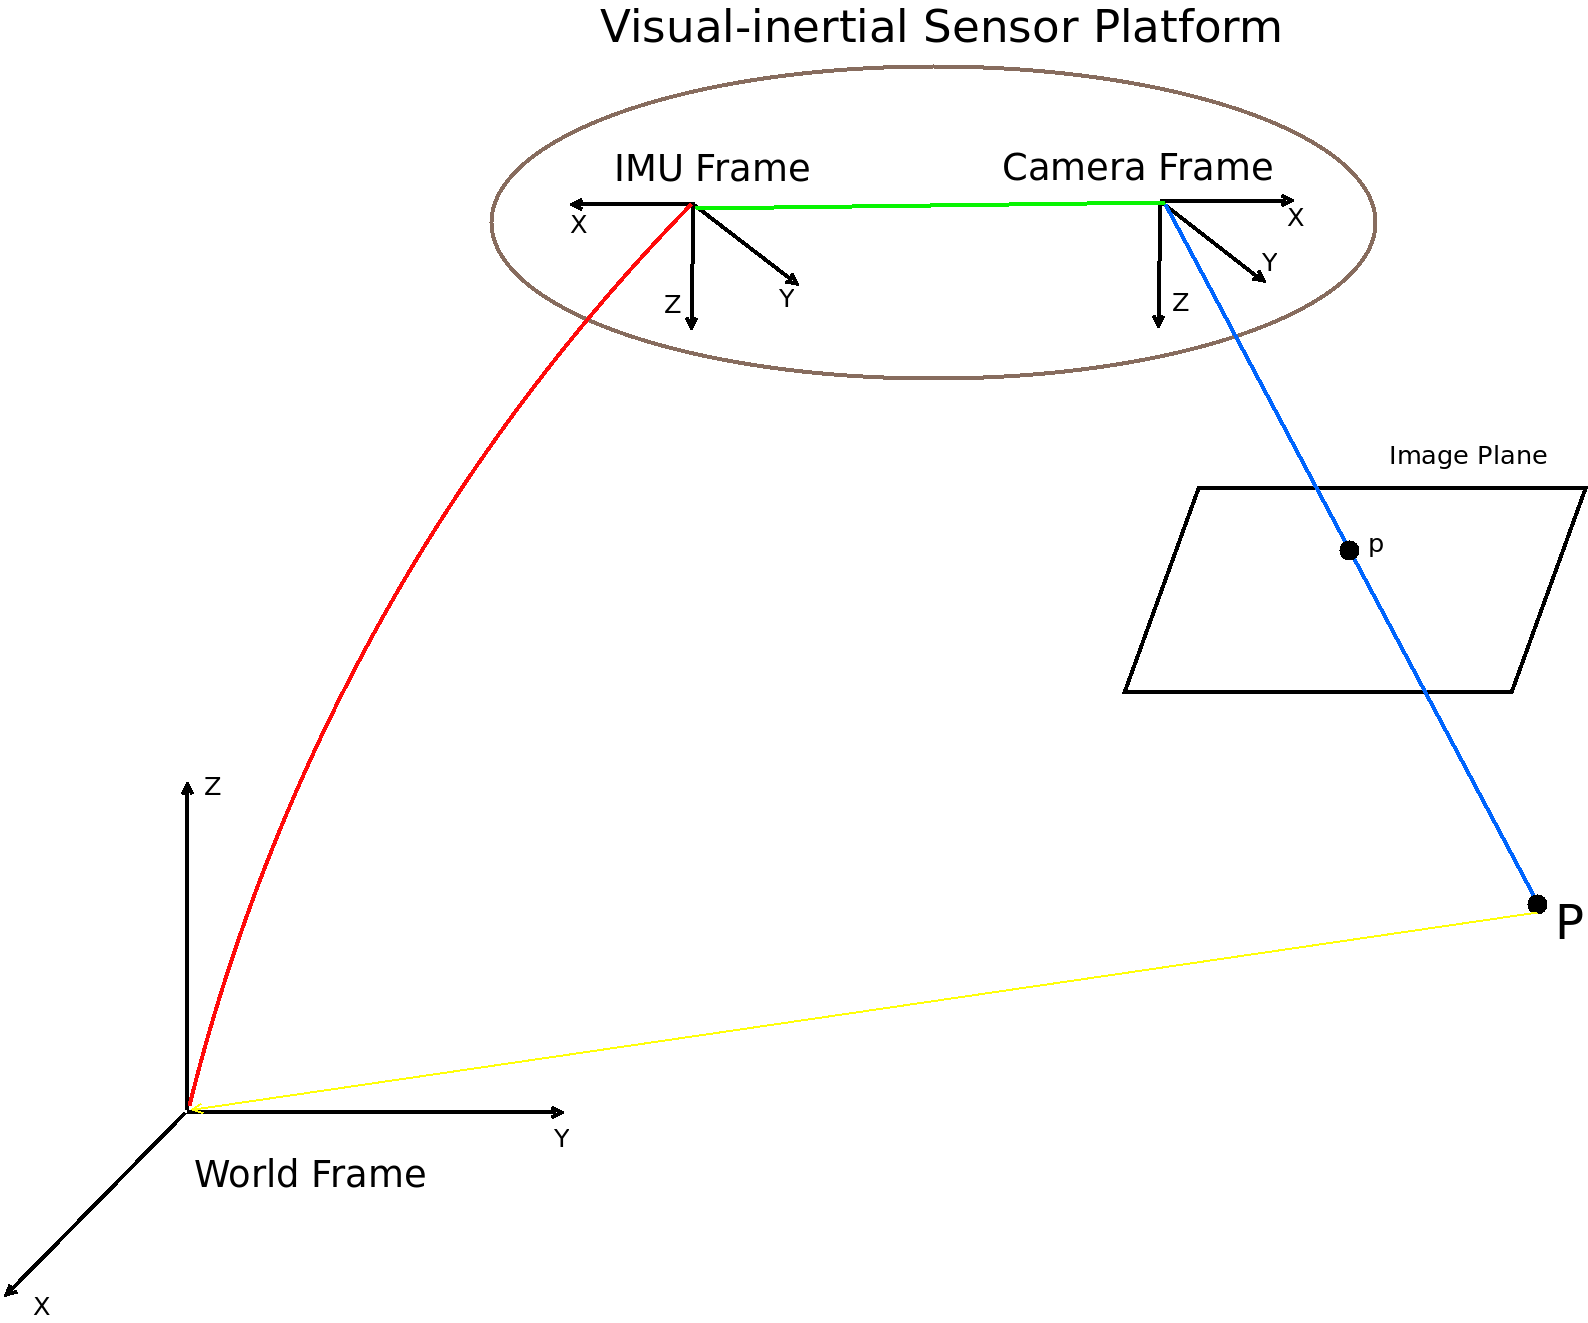
\includegraphics[width=0.8\textwidth]{CONTENT/Figure/Figure2-1_World.png}
    \caption{This figure shows the connection among the world frame $\W$, the IMU frame $\I$ and the camera frame $\C$. Green line shows the transformation between the camera and IMU, which can be pre-calibrated. Red line is the pose of IMU in the world frame. The camera frame observes point $\textbf{p}$ of object P in the image plane, and it connects a object P by blue line. The coordinate of object P in the world frame is presented as yellow line.}
    \label{fig:fig2-1}
\end{figure}

Visual-inertial odometry (VIO)~\cite{li2011consistency}, literally, is an odometry system, which receives environment information by visual (camera) and inertial (IMU) sensors. VIO is similar with the well-known visual odometry (VO) problem \cite{nister2004visual}, with an additional IMU sensor. VIO tries to estimate agent's pose while the agent moves in the environment. One major difference between odometry and SLAM algorithm is that odometry system usually does not build a map, whereas SLAM algorithm localizes and constructs a map at the same time.

To setup a VIO system, we need to first define the world representations. Globally, we have a world frame $\W$; world frame $\W$ is set to a right-handed Cartesian coordinate system that every objects has an absolute pose (translation and rotation). Each sensor has its own local frame, \ie, IMU frame $\I$ and camera frame $\C$, which is also defined as a right-handed Cartesian coordinate system. Every time sensors obtain observations within their own local frame, we estimate the pose of those sensors in world frame $\W$ by integrating these measurements over time. Figure \ref{fig:fig2-1} shows the overall world representations.

In this master thesis, we use following notations,
\begin{itemize}
\item {We denote scalars as $a, b, c$, vectors as $\textbf{a}, \textbf{b}, \textbf{c}$, matrices as $\mA, \mB, \mC$, and frames as $\A, \B, \C$.}
\item {We denote measurement $\textbf{m}$ in a particular frame $\F$ as $\textbf{m}_{\F}$. To further simplify, any parameter that is \textbf{not} in the world frame will be denoted particularly. For example, the translation $\textbf{p}$ in the camera frame will be denoted as $\textbf{p}_{\C}$, and the translation $\textbf{p}$ in the world frame will be denoted as $\textbf{p}$. }
\item {A general translation $\textbf{t}$ should express a translation from point $A$ to point $B$ in frame $\C$, which is denoted as $\textbf{t}^{AB}_{\C}$. In order to simplify our notations, we denote a point $\textbf{p}$ in frame $\A$ as $\textbf{p}_{\A}$ if this point is the translation $\textbf{t}^{OP}_{\A}$, where $O$ is origin of frame $\A$, and $\textbf{p} = P$. This holds same for vectors, which means we can directly use a point $\textbf{p}$ to represent a vector from origin to $\textbf{p}$.}
\item {A general rotation is either expressed in a quaternion $\textbf{q}$ or a rotation matrix $\mR$. To clarify our notations, here we use quaternion $\textbf{q}$ as an example. A quaternion is an orientation operation from frame $\B$ to frame $\A$, and it is denoted as $\textbf{q}_{\A\B}$  in this thesis. Note that if such a operation is from world frame $\W$ to some frame $\B$, we omit both frames for simplification, \ie, $\textbf{q}_{\W\B} \triangleq \textbf{q}$.}
\item {We use hat operator to represent the estimation of state, \ie, $\hat{\vec{x}}$ is the estimation of state $\vec{x}$.}
%TODO: Add more notations when necessary
\end{itemize}

\section{Filter Versus Keyframe}
\label{sec:FVK}

\begin{figure}
\centering
	\begin{subfloat}[Filter]{
		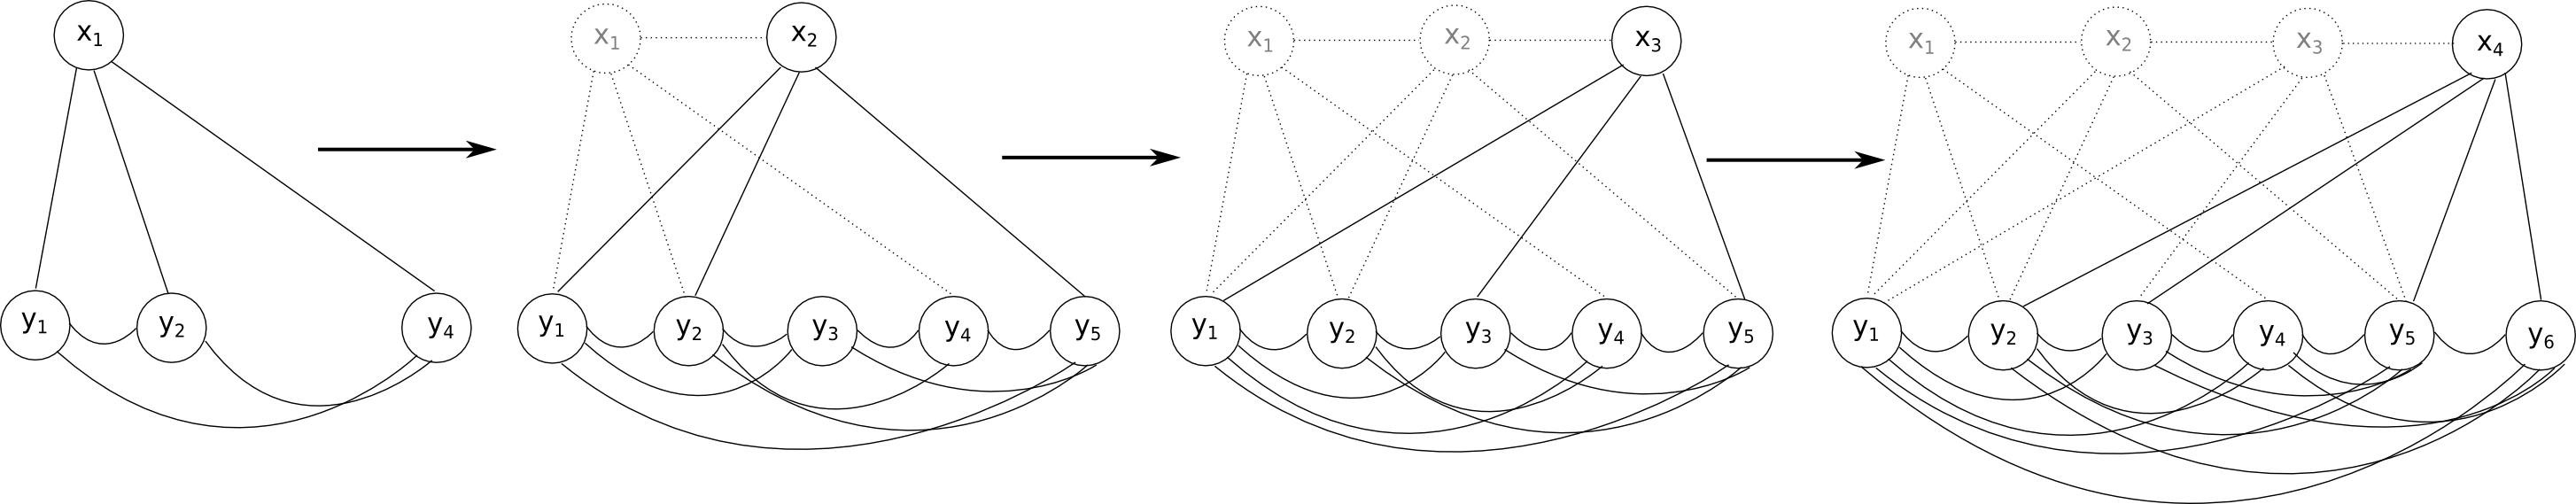
\includegraphics[width=0.8\textwidth]{CONTENT/Figure/Figure2-2-a.png}
		\label{fig:fig2-2-a}}
	\end{subfloat}
	
	%\hspace*{\fill} % separation between the subfigures
	
	\begin{subfloat}[Keyframe-based BA]{
		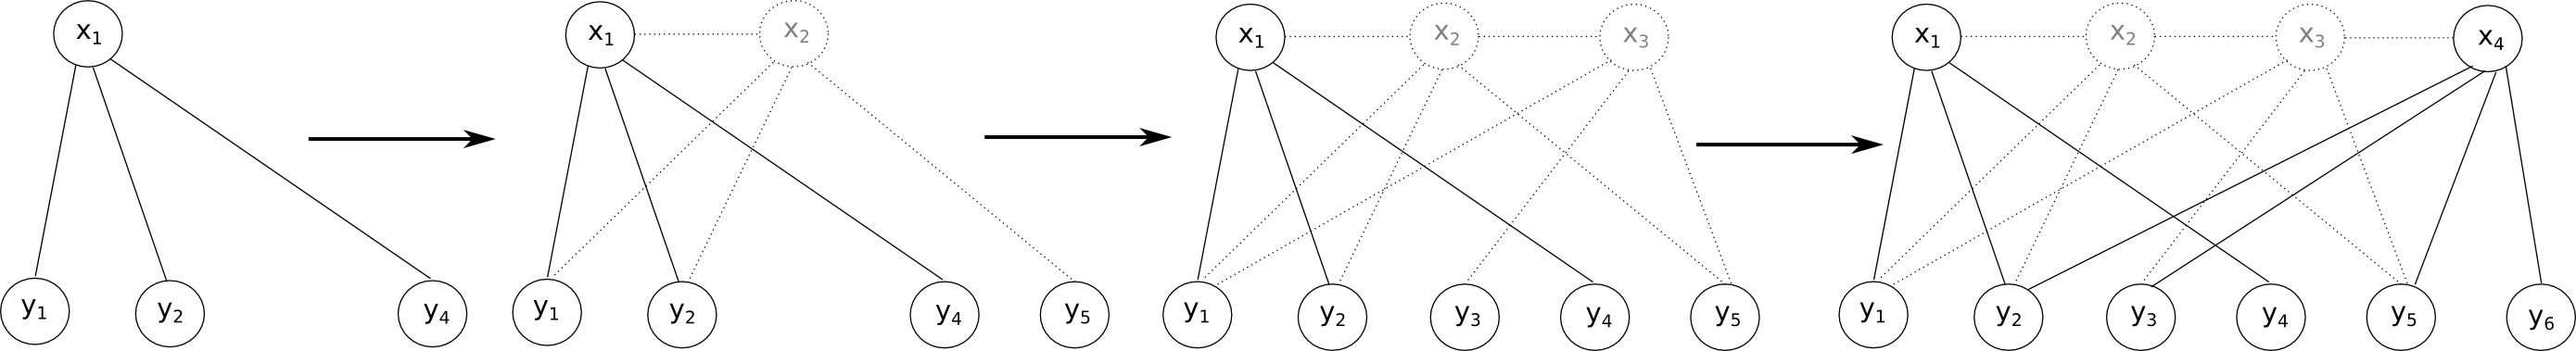
\includegraphics[width=0.8\textwidth]{CONTENT/Figure/Figure2-2-b.png}
		\label{fig:fig2-2-b}}
	\end{subfloat}
	
	%\hspace*{\fill} % separation between the subfigures
	
	\caption{(a) Filter method for SLAM. (b) Keyframe-based Bundle Adjustment (BA) for SLAM. We denote the $i^{th}$ camera position as $\textbf{x}_i$,  $i^{th}$ image feature as $\textbf{y}_i$. We connect the line between camera and image feature if this feature is observed by this camera, the vanished observations is presented as dotted line, and the vanished camera is expressed as grey font. Both graph changes as time goes on from left to right. One can see from (a) that though only the latest camera pose is reserved, the edges between features are increasing exponentially. (b) stores some of former camera poses (keyframe) (\ie, $\textbf{x}_1$ and $\textbf{x}_4$) by keeping graph stay sparsity. } 
	\label{fig:fig2-2}
\end{figure}

It is important to note that though this thesis focuses on visual-inertial odometry for small workspaces, we still intend to keep the possibility to extend our system to a general, scalable, and efficient SLAM system. SLAM system usually has two parallel processes, one is for localization and another is for mapping, the crucial point of building such a system is to keep both processes efficient. There are two general frameworks in visual SLAM: filter-based method and keyframe-based method. In this section, we will discuss whether filter-based method or keyframe-based method is more suitable for our case.

Filter-based SLAM \cite{davison2007monoslam, eade2007monocular, davison2003real} uses \textit{extended Kalman filter} (EKF) to propagate state and update the state covariance. In each step, the system obtains the current estimation of camera pose and landmark positions (3D points) by marginalising all former information. This marginalization step usually eliminates the former pose and adds new connections to image features. As shown in Figure~\ref{fig:fig2-2-a}, the size of graph will not grow very fast as time flows, since the former pose has been eliminated and features in environment is limited. However, once the system moves to large scale scene, it will consume more time to optimize the poses and landmarks as the graph tends to be fully-connected. 
   
Keyframe-based SLAM \cite{klein2007parallel, mourikis2007multi, forster2014svo, engel2014lsd, mur2015orb} applies \textit{bundle adjustment} (BA) on keyframes to update the map. In keyframe-based SLAM, it stores some historical poses (keyframes) and image feature points to proceed a BA step. The chosen of keyframes varies from different implementations, and the idea is to choose a frame that is not very close to the last keyframe, in case that the information might be redundant. In Figure~\ref{fig:fig2-2-b}, the graph stays sparse as the number of poses and features increases. The drawback might be that the behaviour of pose estimation is inadequate as it ignores some former information.

In \cite{strasdat2010real}, they have shown that the computational cost for keyframe BA is $O(m^2 \cdot n)$, and for filter method is $O(n^3)$, where $m$ is the number of key frames, and $n$ is the number of landmarks. They conclude that keyframe-based SLAM is slightly better than filter-based SLAM with their experiment settings, especially when scale of scene becomes larger so that the number of landmarks is far more larger than keyframes.

In this master thesis, we choose keyframe-based method for the visual part and filter method for the IMU integration part. Since we do not keep former information (\eg, image features or landmarks) in integration step, filter method is more efficient whereas each filter step can be regarded as an single optimization step. The reason that we use keyframe-based method for visual part is that we intend to improve the scalability of our system. Moreover the results from IMU integration can be a good compensation in case of the lack of pose estimation in keyframe-based BA.


%% This is an example first chapter.  You should put chapter/appendix that you
%% write into a separate file, and add a line \include{yourfilename} to
%% main.tex, where `yourfilename.tex' is the name of the chapter/appendix file.
%% You can process specific files by typing their names in at the 
%% \files=
%% prompt when you run the file main.tex through LaTeX.
\chapter{Background on Quaternion Algebra}
\label{chap:background}

One important task for this master thesis is to integrate IMU data over the time in order to estimate camera poses (\eg, translations and orientations). By assuming a fixed movement model, it is straightforward to integrate translations in Cartesian space, however since rotational parameter (\eg, Euler angle, rotation matrix, or quaternion) is often represented in manifold, it is often non-trivial to integrate orientations in manifold space. In this chapter, we introduce the quaternion and the quaternion algebra, and then explore the way to operate quaternion over time. General approaches to integrating quaternion over time is given at last.

\section{Definition of Quaternion}
\label{sec:def_of_quat}

A quaternion $Q$ is defined as
\begin{equation}\label{q1}
	Q = q_w + q_xi + q_yj + q_zk,
\end{equation}
where $\{q_w,q_x,q_y,q_z\} \in \mathbb{R}$, and $\{i,j,k\}$ are three imaginary unit lengths, \ie, $i^2=j^2=k^2=ijk=-1$.

In most cases, we represent a quaternion $Q$ as a four-element vector $\textbf{q}$ with respect to above four real numbers $\{q_w,q_x,q_y,q_z\}$, \ie,
\begin{equation}\label{q2}
	\mathbf{q} \triangleq \left[q_w \ \mathbf{q}_v\right]^T = \left[q_w \ q_x \ q_y \ q_z \right]^T,
\end{equation}
where $q_w$ is the real part of $\textbf{q}$, and $vec{q}_v$ is a 3-vector to represent imaginary part of $\textbf{q}$. 

Note that there are two different conventions of quaternion $\textbf{q}$, \textit{Hamilton} way ~\cite{hamilton1844ii} and \textit{JPL} way~\cite{breckenridge1999quaternions}. In Hamilton convention, the real part $q_w$ is the first component of $\textbf{q}$, \ie, $\left[q_w \ \mathbf{q_v}\right]$, whereas in \textit{JPL way}, the real part is the fourth component, \ie, $\left[\mathbf{q_v} \ q_w\right]$. To avoid confusions, and considering Hamilton way is more common to use, especially for implementation~\cite{guennebaud2010eigen, hess2007essential}, we use \textbf{Hamilton way} to represent quaternions throughout the rest of this thesis. 

\section{Properties of Quaternion}
\label{sec:prop_of_quat}

In this section, we introduce the properties of quaternion. 

\textbf{\textit{Summation}} We start with the summation of two quaternions \textbf{q} and \textbf{p}
\begin{equation}\label{q7}
\vec{q} + \vec{p} = \left[q_w+p_w \ \mathbf{q}_v+\mathbf{p}_v\right]^T = \left[q_w+p_w \ q_x+p_x \ q_y+p_y \ q_z+p_z \ \right]^T.
\end{equation}

\textbf{\textit{Product}} We use operator $\otimes$ to denote the product operation on quaternions, which gives
\begin{equation}\label{q3}
	\vec{q} \otimes \vec{p} = \begin{bmatrix}
							  	p_wq_w-p_xq_x-p_yq_y-p_zq_z \\
							  	p_wq_x+p_xq_w+p_yq_z-p_zq_y \\
							  	p_wq_y-p_xq_q+p_yq_w+p_zq_x \\
							  	p_wq_z-p_xq_y-p_yq_z+p_zq_w 
							  \end{bmatrix}.
\end{equation}

The product of two quaternions can be expressed as two equivalent matrix products
\begin{equation}\label{q4}
	\vec{q_1} \otimes \vec{q_2} = Q_1^+\vec{q_2}
\end{equation}
with
\begin{equation}\label{q5}
	Q_1^+ = q_w\ones + \begin{bmatrix}
							  	0 &
							  	-\vec{q_v}^T\\
							  	\vec{q_v} &
							  	[\vec{q_v}]_\times
							  \end{bmatrix},
\end{equation}
where $[\vec{q}_v]_\times$ represents the cross-product matrix of $\vec{q}_v$. The cross-product matrix of a 3-vector $\vec{v}$ is defined by
\begin{equation} \label{q17}
	[\vec{v}]_\times =  \begin{bmatrix}
							0 & -v_z & v_y \\
							v_z & 0 & -v_x \\
							-v_y & v_x & 0 
						\end{bmatrix}.
\end{equation}
Note that the quaternion product is not commutative, \ie, 
\begin{equation}
	\vec{p} \otimes \vec{q} \neq \vec{q} \otimes \vec{p}.
\end{equation}
However it is associative, and distributive over sum, \ie,
\begin{equation} \label{q26}
	\vec{p} \otimes (\vec{q} \otimes \vec{k}) = (\vec{p} \otimes \vec{q}) \otimes \vec{k}
\end{equation}
\begin{equation} \label{q27}
	\vec{p} \otimes (\vec{q} + \vec{k}) = \vec{p} \otimes \vec{q} + \vec{p} \otimes \vec{k}
\end{equation}
\begin{equation} \label{q28}
	(\vec{q} + \vec{k}) \otimes \vec{p} = \vec{q} \otimes \vec{p} + \vec{k} \otimes \vec{p}.
\end{equation}

\textbf{\textit{Conjugate}} The conjugate of a quaternion $\vec{q}^*$ is defined by
\begin{equation}\label{q6}
	\vec{q}^* \triangleq q_w - \vec{q_v} = \left[ q_w \ - \vec{q_v} \right]^T.
\end{equation}

\textbf{\textit{Identity}} An identity quaternion \textbf{q} is defined as, for any given quaternion \textbf{p}, $\vec{q} \otimes \vec{p} = \vec{p} \otimes \vec{q} = \vec{p}$. An identical quaternion \textbf{q} satisfies that
\begin{equation}\label{q8}
	\vec{q} = \left[1 \ 0 \ 0 \ 0 \right]^T.
\end{equation}
In this master thesis, we denote identity quaternion as $\vec{q}_{\ones}$.

\textbf{\textit{Norm}} The norm of a quaternion $\norm{\vec{q}}$ is defined similar to the norm of a vector, which is
\begin{equation}\label{q9}
	\norm{\vec{q}} = \sqrt{q_w^2+q_x^2+q_y^2+q_z^2}.
\end{equation}

\textbf{\textit{Inverse}} The inverse of a quaternion $\vec{q}^{-1}$ is defined as
\begin{equation}\label{q10}
	\vec{q}^{-1} = \vec{q}^* / \norm{\vec{q}},
\end{equation}
which leads to
\begin{equation}\label{q11}
	\vec{q}^* \otimes \vec{q}^{-1} = \vec{q}^{-1} \otimes \vec{q}^*  = \vec{q}_{\mathbb{I}}.
\end{equation}

\textbf{\textit{Unit quaternion}} The norm of a unit quaternion $\norm{\vec{q}}$ is $1$, and the inverse of such a unit quaternion is equal to the conjugate of this quaternion
\begin{equation}\label{q12}
	\vec{q}^{-1} = \vec{q}^*.
\end{equation}

\textbf{\textit{Pure quaternion}} A pure quaternion $\vec{q}$ is defined as
\begin{equation}\label{q13}
	\vec{q} = \left[0 \ \vec{q}_v \right]^T = \left[0 \ q_x \ q_y \ q_z \right]^T.
\end{equation}

Let pure quaternion $\vec{q} = \theta\vec{u}$, where $\theta = \norm{\vec{q}}$, we can compute the exponential of $\vec{q}$ with the help of Euler formula
\begin{equation}\label{q14}
	\mathrm{e}^{\vec{q}} = \mathrm{e}^{\theta\vec{u}} = \cos{\theta} + \vec{u}\sin{\theta} = \left[\cos{\theta} \ \vec{u}\sin{\theta} \right]^T,
\end{equation}
which is still a quaternion, and moreover $\mathrm{e}^{\vec{q}}$ is a unit quaternion because its norm satisfies $\norm{\mathrm{e}^{\vec{q}}}^2 = \cos{\theta}^2 + \sin{\theta}^2 = 1$.

\section{Quaternions and Rotation operations}
\label{sec:quat_and_rot}

We discuss the relationship between quaternions and rotation operations by first introducing rotation vector $\vec{v}$. 

Given a rotation vector $\vec{v} = \phi\vec{u}$, where $\phi$ is the norm of $\vec{v}$ and $\vec{u}$ is a unit vector, we can rotate a vector $\vec{x}$ by an angle $\phi$ around the axis $\vec{u}$ following right-handed rule, and obtain a new vector $\vec{x^{\prime}}$
\begin{equation}\label{q15}
	\vec{x^{\prime}} = \vec{x}_{||} + \vec{x}_{\bot}\cos{\phi} + (\vec{u} \times \vec{x})\sin{\phi},
\end{equation}
where $\vec{x}_{||} = (\vec{x} \cdot \vec{u})\vec{u}$ is the component parallel to $\vec{x}$, and $\vec{x}_{\bot} = -\vec{u} \times (\vec{u} \times \vec{x})$ is the component perpendicular to $\vec{x}$, therefore $\vec{x} = \vec{x}_{||} + \vec{x}_{\bot}$. This formula is known as \textit{vector rotation formular} or \textit{Rodrigues formula}.

Then we can define a rotation matrix $\mR$ by rotation vector $\vec{v} = \phi\vec{u}$ with the help of Equation (\ref{q17}) as
\begin{equation}\label{q16}
	\mR = \mathrm{e}^{[\vec{v}]_\times}.
\end{equation}
We can rotate a vector $\vec{x}$ by an angle $\phi$ around the axis $\vec{u}$ using $\mR$ in a clean way
\begin{equation}\label{q18}
	\vec{x^{\prime}} = \mR\vec{x},
\end{equation}
furthermore one can show that result in Equation (\ref{q18}) is equivalent with the result in Equation (\ref{q15}) \cite{wiki:rotationformula}. 

Constructing a unit quaternion $\vec{q}$ by Equation (\ref{q14}) with a rotation vector $\vec{v} = \phi\vec{u}$ as
\begin{equation}\label{q19}
	\vec{q} = \mathrm{e}^{\vec{v}/2} = \begin{bmatrix}
											\cos{\phi / 2}  \\ \vec{u}\sin{\phi / 2} 
									  \end{bmatrix},
\end{equation}
we can rotate a vector $\vec{x}$ by an angle $\phi$ around the axis $\vec{u}$
\begin{equation}\label{q20}
	\vec{x^{\prime}} = \vec{q} \otimes \vec{x} \otimes \vec{q}^{*}.
\end{equation}

We then show $\vec{x^{\prime}}$ in Equation (\ref{q20}) is equivalent with $\vec{x^{\prime}}$ in Equation (\ref{q15}). First we transferred the vector $\vec{x}$ into pure quaternion form as
\begin{equation}\label{q21}
	\vec{x}_q = \left[0 \ \vec{x} \right]^T,
\end{equation}
then we rewrite formula (\ref{q20}) as
\begin{equation}\label{q22}
\begin{bmatrix}
0  \\ \vec{x^{\prime}} 
\end{bmatrix}
=
\begin{bmatrix}
\cos{\phi / 2}  \\ \vec{v}\sin{\phi / 2} 
\end{bmatrix}
\otimes
\begin{bmatrix}
0  \\ \vec{x} 
\end{bmatrix}
\otimes
\begin{bmatrix}
\cos{\phi / 2}  \\ -\vec{v}\sin{\phi / 2}  
\end{bmatrix}.
\end{equation}
Expanding it by Equation (\ref{q3}), it is easily to show that
\begin{equation}\label{q23}
	\vec{x^{\prime}} = \vec{x}_{||} + \vec{x}_{\bot}\cos{\phi} + (\vec{u} \times \vec{x})\sin{\phi},
\end{equation}
which is exactly Equation (\ref{q15}).

To summarize here, we can construct a quaternion $\vec{q}$ or a rotation matrix $\mR$ by any rotation vector $\vec{v} = \phi\vec{u}$, we denote such a quaternion as $\vec{q} \{ \vec{v} \}$ and rotation matrix as $\mR \{ \vec{v} \}$ respectively. A rotation operation of a vector $\vec{x}$ related to $\vec{v}$ can either be expressed as a quaternion $\vec{q} \{ \vec{v} \} \otimes \vec{x} \otimes \vec{q} \{ \vec{v} \}^{*}$, or as a rotation matrix $\mR \{ \vec{v} \}\vec{x}$. Note that we simplify $\mR \{ \vec{v} \}$ to $\mR$, and/or $\vec{q} \{ \vec{v} \}$ to $\vec{q}$ in the rest of this master thesis.

It is also easy to show the conversion from a rotation matrix $\mR$ to a quaternion $\vec{q}$, which we use in this thesis. Knowing that
\begin{equation}\label{q24}
	\vec{q} \otimes \vec{x} \otimes \vec{q}^{*} = \mR\vec{x},
\end{equation}
we can construct $\mR = \mR \{ \vec{q} \}$ by
\begin{equation}\label{q25}
\mR = \begin{bmatrix}
		q_w^2+q_x^2-q_y^2-q_z^2 & 2(q_xq_y-q_wq_z) & 2(q_xq_z+q_wq_y) \\
		2(q_xq_y+q_wq_z) & q_w^2-q_x^2+q_y^2-q_z^2 & 2(q_yq_z-q_wq_x)\\
		2(q_xq_z-q_wq_y) & 2(q_yq_z+q_wq_x) & q_w^2-q_x^2-q_y^2+q_z^2 \\
	  \end{bmatrix}.
\end{equation} 

The conversion from rotation matrix to quaternion, which is beyond the content of this thesis, can be found in \cite{van2005quaternion}.

\section{Quaternion Differentiation}
\label{sec:timed_on_quat}

We introduce the differentiation on quaternion by first define
\begin{equation}\label{q29}
	\vec{q}(t+\Delta t) \triangleq \vec{q}(t) \otimes \Delta\vec{q},
\end{equation}
where $\vec{q}(t)$ is the quaternion at time $t$ and $\Delta\vec{q}$ is quaternion transformation within a small period time $\Delta t$. 

One can expand $\Delta\vec{q}$ by Taylor expansions with Equation (\ref{q19}) to
\begin{equation}\label{q30}
	\Delta\vec{q} = \begin{bmatrix} 1 \\ \dfrac{1}{2}\Delta{\vec{\theta}} \end{bmatrix} + O(\norm{\Delta{\vec{\theta}}}^2),
\end{equation}
where $\Delta{\vec{\theta}}$ is a angular vector corresponding to $\Delta\vec{q}$. In fact, the angular rate $\vec{\omega}$ at time $t$ is defined as
\begin{equation}\label{q31}
	\vec{\omega} (t) \triangleq \lim_{\Delta{t} \rightarrow 0}\dfrac{\Delta{\vec{\theta}}}{\Delta{t}},
\end{equation}
which is one of measurements we can obtain from IMU sensor.

By definition of the derivative, we can obtain the time-derivative $\dot{\vec{q}}$ of quaternion $\vec{q}$ as
\begin{equation} \label{q32} 
	\dot{\vec{q}} = \dfrac{d\vec{q}(t)}{dt} \triangleq \lim_{\Delta{t} \rightarrow 0} \dfrac{\vec{q}(t+\Delta t) - \vec{q}(t)}{\Delta{t}},
\end{equation}
which follows
\begin{equation} \label{q33} 
\begin{split}
	\dot{\vec{q}} \triangleq & \lim_{\Delta{t} \rightarrow 0} \dfrac{\vec{q}(t+\Delta t) - \vec{q}(t)}{\Delta{t}} \\
	=& \lim_{\Delta{t} \rightarrow 0} \dfrac{\vec{q} \otimes \Delta\vec{q} - \vec{q}}{\Delta{t}} \\
	=& \lim_{\Delta{t} \rightarrow 0} \dfrac{\vec{q} \otimes (\begin{bmatrix} 1 \\ \dfrac{1}{2}\Delta{\vec{\theta}} \end{bmatrix} - \begin{bmatrix} 1 \\ 0 \end{bmatrix})}{\Delta{t}} \\
	=& \frac{1}{2}\vec{q} \otimes \begin{bmatrix} 0 \\ \vec{\omega} \end{bmatrix} 
\end{split}.
\end{equation}
Here we simplify $\vec{q}(t)$ to $\vec{q}$. Then we can obtain the time-derivative on quaternion by writing angular rate into pure quaternion form (\ref{q13}), which is
\begin{equation} \label{q34} 
	\dot{\vec{q}} = \frac{1}{2}\vec{q} \otimes \vec{\omega}.
\end{equation}				  

\section{Time-integration on Quaternion}
\label{sec:timei_on_quat}

To integrate quaternion over time, we explore the relationship between $\vec{q}(t_n)$ and $\vec{q}(t_{n+1})$ where $t_n = n\Delta{t}$. Expanding $\vec{q}(t_{n+1})$ using Taylor series, we have
\begin{equation} \label{q35} 
	\vec{q}(t_{n+1}) = \vec{q}(t_n) + \dot{\vec{q}}(t_n)\Delta{t} + \frac{1}{2!}\ddot{\vec{q}}(t_n)\Delta{t}^2 + \frac{1}{3!}\dddot{\vec{q}}(t_n)\Delta{t}^3+\dots.
\end{equation}

Assume that the second order derivative of rotational rate is zero, which is $\ddot{\vec{\omega}} = 0$, we have
\begin{align} 
	\label{q36} 
	\dot{\vec{q}}(t_{n+1}) &= \frac{1}{2}\vec{q}(t_{n}) \otimes \vec{\omega}(t_{n}) \\
	\label{q37} 
	\ddot{\vec{q}}(t_{n+1}) &= \frac{1}{2^2}\vec{q}(t_{n}) \otimes \vec{\omega}^2(t_{n})+\frac{1}{2}\vec{q}(t_{n}) \otimes \dot{\vec{\omega}} \\
	\label{q38} 
	\dddot{\vec{q}}(t_{n+1}) &= \frac{1}{2^3}\vec{q}(t_{n}) \otimes \vec{\omega}^3(t_{n}) + \frac{1}{4}\vec{q}(t_{n}) \otimes \dot{\vec{\omega}}\vec{\omega}(t_{n}) + \frac{1}{2}\vec{q}(t_{n}) \otimes \vec{\omega}(t_{n})\dot{\vec{\omega}} \\
	 \vdots & \nonumber 
\end{align}
and so forth and so on. We then get the result of time integration by taking Equation (\ref{q36}), (\ref{q37}), and (\ref{q38}) back into Equation (\ref{q35}).

We hereby uses a stronger assumption that angular rate $\vec{\omega}(t_{n})$ remains constant during a small time period $\Delta{t}$, which is $\dot{\vec{\omega}} = 0$. Considering the sampling rate of IMU sensor is usually high (> 100 [Hz]), this assumption is actually quite accurate in practice. Moreover it gives us a cleaner expression of the quaternion time integration formula. 

Given $\dot{\vec{\omega}} = 0$, we can get
\begin{equation} \label{q39} 
	\vec{q}_{n+1} = \vec{q}_n \otimes (1+\frac{1}{2}\vec{\omega}_n\Delta{t}+\frac{1}{2!}(\frac{1}{2}\vec{\omega}_n\Delta{t})^2+\frac{1}{3!}(\frac{1}{2}\vec{\omega}_n\Delta{t})^3+\frac{1}{4!}(\frac{1}{2}\vec{\omega}_n\Delta{t})^4+\dots).
\end{equation}
Here we regard $\vec{q}$ and $\vec{\omega}$ as series, which is exactly
\begin{equation} \label{q40} 
	\vec{q}_{n+1} = \vec{q}_n \otimes \mathrm{e}^{\vec{\omega}\Delta{t}/2}.
\end{equation}
We can rewrite it by Equation (\ref{q19}) as
\begin{equation} \label{q41} 
	\vec{q}_{n+1} = \vec{q}_n \otimes \vec{q}\{ \vec{\omega}_n\Delta{t} \},
\end{equation}
which is called \textbf{\textit{Zeroth order forward integration}} of quaternion over time.

We can obtain \textbf{\textit{Zeroth order backward integration}} by assuming the angular rate remains $\vec{\omega}_{n+1}$ within $\Delta{t}$, then we have
\begin{equation} \label{q42} 
	\vec{q}_{n+1} = \vec{q}_n \otimes \vec{q}\{ \vec{\omega}_{n+1}\Delta{t} \},
\end{equation}
and \textbf{\textit{Zeroth order midward integration}} by assuming the angular rate holds $\bar{\vec{\omega}}_{n+1} =(\vec{\omega}_{n}+ \vec{\omega}_{n+1})/2$ within $\Delta{t}$, which is
\begin{equation} \label{q43} 
	\vec{q}_{n+1} = \vec{q}_n \otimes \vec{q}\{ \bar{\vec{\omega}}_{n}\Delta{t} \}.
\end{equation}

Though not used in this master thesis, we notice that \cite{trawny2005indirect} gives \textbf{\textit{First order integration}} by assuming angular rate is linear with time, \ie, $\dot{\vec{\omega}} = \frac{\vec{\omega}_{n+1} - \vec{\omega}_{n}}{\Delta{t}}$, which is precisely
\begin{equation} \label{q44} 
	\vec{q}_{n+1} = \vec{q}_n \otimes \vec{q}\{ \bar{\vec{\omega}}_{n}\Delta{t} \} + \frac{\Delta{t}^2}{48}\vec{q}_n\otimes(\vec{\omega}_n \otimes \vec{\omega}_{n+1} - \vec{\omega}_{n+1} \otimes \vec{\omega}_{n}) + \dots
\end{equation}
in our quaternion convention.
% %% This is an example first chapter.  You should put chapter/appendix that you
%% write into a separate file, and add a line \include{yourfilename} to
%% main.tex, where `yourfilename.tex' is the name of the chapter/appendix file.
%% You can process specific files by typing their names in at the 
%% \files=
%% prompt when you run the file main.tex through LaTeX.
\chapter{Generalized Higher Order Power Method for Hypergraph Matching}
\section{Power Method}
\section{Higher Order Power Method}
\section{$l_p$ Generalized Higher Order Power Method}

%\include{CONTENT/motivation}
%% This is an example first chapter.  You should put chapter/appendix that you
%% write into a separate file, and add a line \include{yourfilename} to
%% main.tex, where `yourfilename.tex' is the name of the chapter/appendix file.
%% You can process specific files by typing their names in at the 
%% \files=
%% prompt when you run the file main.tex through LaTeX.
\chapter{Modular Sensor Fusing}
\label{chap:sensor_fusing}

In previous chapter, we learned how to represent each frame and analysed the difference between filter method and keyframe BA method for our odometry system. We also learned quaternion algebra and basic approaches for quaternion integration and derivative over the time under some general assumptions. In this chapter, we will explore the details of our sensor fusing approach, which uses so called \textit{IMU loose integration framework}~\cite{weiss2012vision}. In such a framework, system propagates states via Kalman filter (KF) based on IMU measurements, and extrasensory (\eg, camera, GPS \etc) data are used in correction step. The computational cost for Kalman-filter-styled approach is usually linear, hence \textit{IMU loose integration framework} provides a better trade-off between computational complexity and accuracy in a real-time robotic navigation system.

\section{Error-state Kalman Filter for IMU Integration}
\label{sec:ESKF_IMU}

The error-state Kalman filter (ESKF) follows the paradigm of Kalman filter, which also has prediction step and correction step. However, ESKF separates system into three different states: true state, nominal state, and error state. Nominal state processes large signal, which is integrable in a non-linear fashion, whereas error state keeps track of error and noise term, which can be integrated in a linear way. The composition of nominal state and error state, and we call it true state, which is the final guess of the system.

The ESKF has several beneficial properties when building a visual-inertial odometry:                                                                                                                                                                                                                                                                                                              
\begin{enumerate}
	\item The computation of Jacobian may be very fast, because the error state is small and all second order products are negligible. This is an important factor building a real-time system.
	\item Fusing visual data with IMU data is straightforward in Kalman filter correction step. One can utilize the tracking result to correct the IMU integration state.
	\item Large signals have been integrated into nominal states, so that we can apply the correction step in a lower rate than prediction step.
\end{enumerate}

The procedure of ESKF in this system can be explained as follows. Firstly, IMU data is integrated into nominal state via numerical integration methods, note that nominal state does not take noise terms or error terms into account, hence nominal state will accumulate errors. The error state then predict the errors and noise terms using normal extended KF paradigm, meaning it will predict the mean and covariance of the error state. In parallel a correction step is performed at a lower rate, the results of visual tracking are used to correct the error state, the error state is then injected into nominal state, which the nominal state becomes the final guess of system at that time point. The system continues until the criterion condition has been met.

We explain the ESKF for IMU integration in this section, and visual sensor as correction data in Section \ref{sec:camera_comple_data}.

%\subsection{Motivation}
%\label{subsec:ESKF_IMU_sub1}

\subsection{System Kinematics}
\label{subsec:ESKF_IMU_sub2}

We denote our true state $\vec{x}_t$ as
\begin{equation}\label{f1}
	\vec{x}_t = \vec{x}_n \oplus \vec{x}_e,
\end{equation}
where $\vec{x}_n$ is the nominal state for large signals, $\vec{x}_e$ is error state for small error/noise signal, and we have used $\oplus$ to denote a general composition step. 

We then introduce position $\vec{p}$, velocity $\vec{v}$, quaternion $\vec{q}$, accelerometer bias $\vec{a}_b$, gyroscope bias $\vec{\omega}_b$ and gravity vector $\vec{g}$ into true state, nominal state and error state respectively. The general composition step can be shown as
\begin{align}
	\vec{p}_t =& \vec{p}_n + \vec{p}_e \\
	\vec{v}_t =& \vec{v}_n + \vec{v}_e \\
	\vec{q}_t \approx& \vec{q}_n \otimes \begin{bmatrix} 1 \\ \vec{\theta}_e / 2 \end{bmatrix} \label{f2}\\
	\vec{a}_{bt} =& \vec{a}_{bn} + \vec{a}_{be} \\
	\vec{\omega}_{bt} =& \vec{\omega}_{bn} + \vec{\omega}_{be} \\ 
	\vec{g}_t =& \vec{g}_n + \vec{g}_e,
\end{align}
note that we derive Equation (\ref{f2}) by the small angle approximation (Equation (\ref{q30})). We apply angular error $\vec{\theta}_e$ instead of quaternion error in error state following classical approaches.

We then construct kinematic equations for true state, which are
\begin{align}
	\label{f18}
	\dot{\vec{p}_t} =& \vec{v}_t \\
	\dot{\vec{v}_t} =& \mR_t(\vec{a}_m - \vec{a}_{bt} - \vec{a}_n) + \vec{g}_t\\
	\dot{\vec{q}_t} =& \frac{1}{2}\vec{q}_t \otimes (\vec{\omega}_m - \vec{\omega}_{bt} - \vec{\omega}_n) \\
	\dot{\vec{a}_{bt}} =& \vec{a}_w \\
	\dot{\vec{\omega}_{bt}} =& \vec{\omega}_{w} \\ 
	\label{f19}
	\dot{\vec{g}_t} =& 0,
\end{align}
where $\vec{a}_m$ and $\vec{\omega}_m$ are the measurements from accelerometer and gyroscope respectively within \textbf{local frame}, $\vec{a}_n$ and $\vec{\omega}_n$ are noises with those measurements, $\vec{a}_w$ and $\vec{\omega}_w$ are white Gaussian noise together with accelerometer and gyroscope bias, and $\mR_t$ is the rotation matrix corresponding to true state quaternion, \ie, $\mR_t \triangleq \mR_t\{ \vec{q} \}$ regarding to Equation (\ref{q25}). We use similar notations in nominal state and error state. 

We obtain kinematic equations for nominal state by cutting off all small signals, which leads to
\begin{align}
	\label{f12}
	\dot{\vec{p}_n} =& \vec{v}_n \\
	\label{f11}
	\dot{\vec{v}_n} =& \mR_n(\vec{a}_m - \vec{a}_{bt}) + \vec{g}_n\\
	\dot{\vec{q}_n} =& \frac{1}{2}\vec{q}_n \otimes (\vec{\omega}_m - \vec{\omega}_{bn})\\
	\dot{\vec{a}_{bn}} =& 0 \\
	\dot{\vec{\omega}_{bn}} =& 0 \\ 
	\label{f13}
	\dot{\vec{g}_n} =& 0,
\end{align}
and the error state with small signals is
\begin{align}
	\label{f3}
	\dot{\vec{p}_e} =& \vec{v}_e \\
	\label{f4}
	\dot{\vec{v}_e} =& \mR_n \left[ \vec{a}_m - \vec{a}_{bn} \right]_{\times} -  \mR_n\vec{a}_{be} + \vec{g}_e - \mR_n\vec{a}_n\\
	\label{f5}
	\dot{\vec{\theta}_e} =& \left[ \vec{\omega}_m - \vec{\omega}_{bn} \right]_{\times} - \vec{\omega}_{be} - \vec{\omega}_{n}\\
	\label{f6}
	\dot{\vec{a}_{be}} =& \vec{a}_w \\
	\label{f7}
	\dot{\vec{\omega}_{be}} =& \vec{\omega}_{w} \\ 
	\label{f8}
	\dot{\vec{g}_e} =& 0. 
\end{align}
It is trivial to derive Equation (\ref{f3}, \ref{f6}, \ref{f7}, \ref{f8}), see Appendix \ref{chap:appendix1} for derivation of Equation (\ref{f4} and \ref{f5}).

\subsection{State Time-integration and Error-state Jacobian}
\label{subsec:ESKF_IMU_sub3}

We propose time-integration equations between any two time stamp $t_n$ and $t_{n+1}$ where we measure the time difference $\Delta{t}$ as $\Delta{t} = t_{n+1} - t_{n}$. In order to simplify our notations, we denote last state parameters as $\vec{x}$, and denote current state parameters as $\vec{x}^{\prime}$, where current state is measured at time stamp $t_{n}$, and last state is measured at $t_{n-1}$. Same notations are set for error state. Therefore, time-integration equations for nominal state for one updating are
\begin{align}
	\vec{p}_n^{\prime} =& \vec{p}_n + \vec{v}_n\Delta{t} + \frac{1}{2}(\mR_n(\vec{a}_m - \vec{a}_{bt}) + \vec{g}_n)\Delta{t}^2 \\
	\vec{v}_n^{\prime} =& \vec{v}_n + (\mR_n(\vec{a}_m - \vec{a}_{bt}) + \vec{g}_n)\Delta{t}\\
	\label{f9}
	\vec{q}_n^{\prime} =& \vec{q}_n \otimes \vec{q}\{(\vec{\omega}_m - \vec{\omega}_{bn})\Delta{t}\}\\
	\vec{a}_{bn}^{\prime} =& \vec{a}_{bn} \\
	\vec{\omega}_{bn}^{\prime} =& \vec{\omega}_{bn} \\ 
	\vec{g}_n^{\prime} =& \vec{g}_n.
\end{align}
We use \textbf{\textit{Zeroth order forward integration}} explained in Section \ref{sec:timei_on_quat} to integrate our state over time, this is also called Euler method in Runge-Kutta numerical integration methods (see Appendix \ref{sec:runge_kutta}).

We integrate our error state in the same manner, except we have truncated second-order signal out. We obtain the integration equations for error state by
\begin{align}
	\vec{p}_e^{\prime} =& \vec{p}_e + \vec{v}_e \Delta{t}\\
	\vec{v}_e^{\prime} =& \vec{v}_e + (\mR_n \left[ \vec{a}_m - \vec{a}_{bn} \right]_{\times} -  \mR_n\vec{a}_{be} + \vec{g}_e)\Delta{t} + \vec{v}_i\\
	\label{f10}
	\vec{\theta}_e^{\prime} =& (\mR_n^T \{ \vec{\omega}_m - \vec{\omega}_{bn} \} \vec{\theta}_e - \vec{\omega}_{be})\Delta{t} + \vec{\theta}_{i}\\
	\vec{a}_{be}^{\prime} =& \vec{a}_{be} + \vec{a}_i\\
	\vec{\omega}_{be}^{\prime} =& \vec{\omega}_{be} + \vec{\omega}_i\\ 
	\vec{g}_e^{\prime} =& \vec{g}_e,
\end{align}
where $\vec{v}_i$, $\vec{\theta}_{i}$, $\vec{a}_i$, and $\vec{\omega}_i$ are random impulses for velocity, angular error, accelerometer bias and gyroscope. Those impulses can be modelled by Gaussian process. We derive Equation (\ref{f10}) by close-formed integration methods described in Appendix \ref{sec:close_integration}.

We then provide the Jacobian of error state $\mJ_{x_e}$ for ESKF prediction step usage
\begin{equation}\label{f14}
	\mJ_{e^\prime e} = \frac{\partial{\vec{x}_e^{\prime}}}{\partial{\vec{x}_e }} = \begin{bmatrix}
	\ones & \ones\Delta{t} & 0 & 0 & 0 & 0 \\
	0 & \ones & \mR_n \left[ \vec{a}_m - \vec{a}_{bn} \right]_{\times}\Delta{t} & \mR_n\Delta{t} & 0 & \ones\Delta{t} \\
	0 & 0 & \mR_n^T \{ \vec{\omega}_m - \vec{\omega}_{bn} \}\Delta{t} & 0 & -\ones\Delta{t} & 0 \\
	0 & 0 & 0 & \ones & 0 & 0 \\
	0 & 0 & 0 & 0 & \ones & 0 \\
	0 & 0 & 0 & 0 & 0 & \ones \\
	\end{bmatrix}.
\end{equation}

Note that partial derivative between true state $\vec{x}_t$ and $\vec{x}_e$ is not identity because we use different parameters to represent orientations, \eg quaternion in true state, angular error in error state. We then give the Jacobian of true state with respect to error state with
\begin{equation}\label{f15}
	\mJ_{t e} = \frac{\partial{\vec{x}_t}}{\partial{\vec{x}_e }} = \begin{bmatrix}
	\ones & 0 & 0 & 0 & 0 & 0 \\
	0 & \ones &0 & 0 & 0 & 0 \\
	0 & 0 & \frac{\partial{\vec{q}_t}}{\partial{\vec{\theta}_e }} & 0 & 0 & 0 \\
	0 & 0 & 0 & \ones & 0 & 0 \\
	0 & 0 & 0 & 0 & \ones & 0 \\
	0 & 0 & 0 & 0 & 0 & \ones \\
	\end{bmatrix}.
\end{equation}
By Equation (\ref{q5}), we have
\begin{align}\label{f16}
	\frac{\partial{\vec{q}_t}}{\partial{\vec{\theta}_e }} &= \frac{1}{2}Q^+(\vec{q})\begin{bmatrix}
	0 & 0 & 0 \\
	1 & 0 & 0 \\
	0 & 1 & 0 \\
	0 & 0 & 1 \\
	\end{bmatrix} \\
	&= \frac{1}{2}\begin{bmatrix}
	-q_x & -q_y & -q_z \\
	q_w & -q_x & q_y \\
	q_z & q_w & -q_x \\
	-q_y & q_x & q_w \\
	\end{bmatrix}. 
\end{align}

\subsection{State Propagation}
\label{subsec:ESKF_IMU_sub4}

Initially, nominal state $\vec{x}_n$ has been set to an initial guess based on the prior knowledge, and there is no error at start, \ie, error state is set to zero. We assume error state $\vec{x}_e$ as a normal distribution, \ie, $\vec{x}_e \sim \mathcal{N}(\hat{\vec{x}_e}, \mSigma)$, where $\mSigma$ denotes the covariance matrix for error state, which helps us to track the uncertainty of error state. Note that $\mSigma$ is initialized to a very small diagonal matrix.

At the certain round, we first obtain the measurements from accelerator and gyroscope, and compute a new nominal state estimation $\hat{\vec{x}_n^\prime}$ from Equation (\ref{f12}) to (\ref{f13}). We then compute error state Jacobian $\mJ_{e^\prime e}^\prime$ by Equation(\ref{f14}), then update the error state and covariance matrix of current error state by
\begin{align} \label{f22}
\hat{\vec{x}_e^\prime} &= \mJ_{e^\prime e}^\prime\hat{\vec{x}_e} \\
\mSigma^\prime &= \mJ_{e^\prime e}^\prime \mSigma (\mJ_{e^\prime e}^\prime)^T,
\end{align}
which is called \textit{prediction step} in ESKF. We omit prime symbol in the next step, \ie current state $\vec{x}$ is replaced by $\vec{x}^\prime$.

We then assume correction measurement $\vec{y}$ from extrasensory data is a non-linear function with additional white Gaussian noise $w \sim \mathcal{N}(0, \mW)$ of our true state, \ie,
\begin{equation}\label{f17}
	\vec{y} = h(\vec{x}_t) + w,
\end{equation}
and the \textit{correction step} of ESKF are as follows
\begin{align}\label{f30}
	\mK &= \mSigma\mH^T(\mH\mSigma\mH^T+\mW)^{-1} \\
	\hat{\vec{x}_e^\prime} &= \mK (\vec{y} - h(\hat{\vec{x}_t})) \\
	\mSigma^\prime &= (\ones - \mK\mH)\mSigma,
\end{align}
where $\mH$ is the Jacobian matrix of measurement function $h(\cdot)$ with respect to error state $\vec{x}_e$ (see Section \ref{subsec:camera_comple_data_sub2}). Note the estimation of true state here is the nominal state since we have not observed the mean of error state. The true state is estimated by Equation (\ref{f1}) and Equation (\ref{f18}) to (\ref{f19}). Depending on the output frequency of extra sensor, \textit{correction step} often happens on a lower rate than \textit{prediction step}. As always, we omit prime symbol in next few steps as state has been refreshed.  

Before the system enters into the next round, we reset error state to initial state, \ie, $\hat{\vec{x}_e} = 0$ in our case. We update covariance matrix $\mSigma$ by
\begin{equation}\label{f20}
	\mSigma^\prime = \mJ_{ge} \mSigma (\mJ_{ge})^T,
\end{equation}
where $\mJ_{ge}$ is Jacobian matrix of updated error state with respect to old error state. $\mJ_{ge}$ is given by
\begin{equation}\label{f21}
	\mJ_{ge} \triangleq \dfrac{\partial{\vec{x}_e^\prime}}{\partial{\vec{x}_e}} = \begin{bmatrix}
	\ones_6 & 0 & 0 \\
	0 & \ones - \left[ \frac{1}{2} \hat{\vec{\theta}_e} \right]_\times & 0 \\
	0 & 0 & \ones_9 \\
	\end{bmatrix},
\end{equation}
where we use $\vec{x}^\prime$ to denote the new state after resetting error state. The Jacobian is identical on all diagonal blocks except angular error term for the assumption we have made in Equation (\ref{q30}). We derive the $\mJ_{ge}$ by two observations, first the true state will not be able to change during the reset of error state; second, the new nominal state is obtained by injecting old error state mean from old nominal state, which the above observation can be transformed into following equations
\begin{align}
	\label{f31}
	\vec{x}_n^\prime \oplus \vec{x}_e^\prime =& \vec{x}_n \oplus \vec{x}_e \\
	\label{f32}
	\vec{x}_n^\prime =& \vec{x}_n \oplus \hat{\vec{x}_e}.
\end{align}
Putting Equation (\ref{f32}) into Equation (\ref{f31}), we have
\begin{equation}
	\vec{q}_e^\prime = (\vec{q}_n \otimes \hat{\vec{q}_e})^* \otimes \vec{q}_n \otimes \vec{q}_e = Q^+(\hat{\vec{q}_e})^*\vec{q}_e.
\end{equation}
By using small angle approximation (Equation (\ref{q5})) and throwing second order term, we can obtain 
\begin{equation}
	\vec{\theta}_e^\prime = -\hat{(\vec{\theta}_e} + (\ones - \left[ \frac{1}{2} \hat{\vec{\theta}_e} \right]_\times)\vec{\theta}_e.
\end{equation}
After derivation of old angular term from both sides, we get 
\begin{equation}
	\dfrac{\partial{\vec{\theta}_e^\prime}}{\partial{\vec{\theta}_e}} = \ones - \left[ \frac{1}{2} \hat{\vec{\theta}_e} \right]_\times,
\end{equation}
which is precisely the term in Equation (\ref{f21}).
\section{Camera as Complementary Sensory Data}
\label{sec:camera_comple_data}

As we discussed in Section \ref{sec:ESKF_IMU}, we need extrasensory data in ESKF \textit{correction step}, and we modelled this sensor as a non-linear measurement of true state $\vec{x}_t$ plus a white Gaussian noise as shown in Equation (\ref{f17}). This sensor in our case should satisfy the following conditions:
\begin{itemize}
\item {This sensor should carry rich information as we need to obtain accurate camera pose estimation from it.}
\item {This sensor, unlike GPS, should work both inside and outside environment as our system is designed for mobile robots.}
\item {This sensor should be light-weight, low-expense and better easy to handle as this is the general requirements for mobile robots.}
\end{itemize}
which lead to our choice --- camera. It is worthy to note that though we treat data in correction step as a black box, it is also possible to choose a multiple sensory platform. However on the one hand, we choose camera not only it satisfies all the above conditions, but also the camera as most commonly-used sensor has been well-investigated and well-understand, which could help us to find multiple possible approaches to solve our problem, \eg, camera pose estimation in our case; on the other hand, multiple extra sensors (\ie, camera+GPS) probably meet some issues such as synchronizing between multiple sensory platforms. Therefore we choose camera as complementary data in this work.

\subsection{Introduction to Monocular Visual Odometry}
\label{subsec:camera_comple_data_sub1}

Visual odometry estimates the camera pose, and it can provide the measurements (\eg, global translation and rotation) we need in ESKF prediction step as the transformation between camera and IMU has been pre-calibrated. We here briefly introduce different types of visual odometry system. There are stereo-based odometry \cite{mei2009constant}, depth-camera odometry \cite{newcombe2011kinectfusion}, however considering we only use single camera in this work, we mainly introduce monocular visual odometry.

A monocular odometry usually works as follows. Initially, the system obtains the first guess of camera's pose by \textit{Homography} \cite{fischler1981random} between two images. After a new image is acquired, the system then tries to find the correspondences among common \textit{landmarks}, where a landmark is defined as the most distinctive object in the real world. Depending on the types of correspondences, we have
\begin{itemize}
\item {\textbf{Feature-based methods} As proposed in \cite{davison2007monoslam, eade2007monocular, klein2007parallel, mur2015orb}, feature-based methods use image features to denote these correspondences, \eg, points are the same if the features corresponding to it are same. The system then reprojects similar points from the last image to the current one using estimated camera pose transformation, errors between points in the current visual frame is called reprojection error.}
\item {\textbf{Direct methods} As proposed in \cite{engel2014lsd}, it uses image intensity (\eg, photometric error) to find such correspondences.}
\item {\textbf{Semi-direct methods} As shown in \cite{forster2014svo}, it uses combinations of image features and image intensities to find correspondences.}
\end{itemize}
After the connections of points  between two images has been established, camera pose is estimated by minimizing the re-projection error or image intensity error.

Building a map based on such odometry is straightforward. A point is recognized as a part of landmark if it has been frequently tracked, and then will be inserted into the map as a recognized "map point"; a map is then constructed by such map points, and normally a batch processing (\eg, bundle adjustment) is used for optimizing the map during mapping process. However, such a technique can also be used for improving the pose estimation quality as we introduced in Section \ref{subsec:camera_comple_data_sub3}.

\subsection{Self-adapt Map Scale}
\label{subsec:camera_comple_data_sub2}

Estimation of camera pose from monocular visual odometry (VO) usually is a good compensation to ESKF IMU integration since global translation is unobservable to IMU integration. Since camera is an angle-sensor, it is impossible to obtain the scale of map \cite{forster2014svo}, \ie, global translation from monocular VO has been scaled up/down with real world scale. Researchers have estimated map scale factor by aligning the first few frames with ground-truth data \cite{forster2014svo}, or initialize map scale by a standard object (\eg, a A4 paer) \cite{davison2007monoslam}, and it is still likely to accumulate scale drift with time goes on. In our framework, since IMU measures under a real world scale, we can propagate the map scale in our ESKF framework by introducing a scale factor in our state. 

We first add the scale factor $\vec{\lambda}$ which contains a 3-vector to represent the scalability with x-axis, y-axis, and z-axis respectively. Now our true state, nominal state, and error state have been changed into
\begin{align}
	\vec{x}_t &= \left[ \vec{p}_t \ \vec{v}_t \ \vec{q}_t \ \vec{a}_{bt} \ \vec{\omega}_{bt} \ \vec{g}_{t} \ \vec{\lambda}_{t} \right]^T \\
	\vec{x}_n &= \left[ \vec{p}_n \ \vec{v}_n \ \vec{q}_n \ \vec{a}_{bn} \ \vec{\omega}_{bn} \ \vec{g}_{n} \ \vec{\lambda}_{n} \right]^T \\
	\vec{x}_e &= \left[ \vec{p}_e \ \vec{v}_e \ \vec{\theta}_e \ \vec{a}_{be} \ \vec{\omega}_{be} \ \vec{g}_{e} \ \vec{\lambda}_{e} \right]^T .
\end{align}
The derivative with $\vec{\lambda}$ with respect to time is easily derived since we assume the scale factor is independent with time, therefore we have
\begin{align}
	\dot{\vec{\lambda}_t} &= 0 \\
	\dot{\vec{\lambda}_n} &= 0 \\
	\dot{\vec{\lambda}_e} &= 0.
\end{align}
It is trivial to make corresponding changes to system kinematic equations (\eg, Equation \ref{f12} to \ref{f18}) and the error state Jacobian (\eg, Equation \ref{f15} and \ref{f16}). The measurement function $h(\cdot)$ of estimated true state $\dot{\vec{x}_t}$ can be derived as
\begin{align}
	\label{f23}
	h(\vec{p}_t) &= \vec{\lambda}_t \odot (\vec{p}_t - \vec{p}_{t0}) + \vec{p}_{t0}\\
	\label{f24}
	h(\vec{v}_t) &= \vec{v}_t\\
	\label{f25}
	h(\vec{q}_t) &= \vec{q}_t\\
	\label{f26}
	h(\vec{a}_{bt}) &= \vec{a}_{bt} \\
	\label{f27}
	h(\vec{\omega}_{bt}) &= \vec{\omega}_{bt} \\ 
	\label{f28}
	h(\vec{g}_t) &= \vec{g}_t \\
	\label{f29}
	h(\vec{\lambda}_t) &= \vec{\lambda}_t,
\end{align}
where $\odot$ is point-wise vector multiplication and $\dot{\vec{p}_{t0}}$ is the camera/IMU position in reference frame, \ie, the position obtained from Homography of first two keyframes. We assume the camera sensor and IMU sensor have identical position for simplification, \ie, $\dot{\vec{p}_t}$ is the estimated camera position in world frame. A more complicated case can be found in \cite{lynen2013robust}.

In Section \ref{sec:ESKF_IMU}, we did not give the explicit expression of $\mH$ in Equation (\ref{f22}). $\mH$ is defined as the Jacobian matrix of extrasensory measurement function $h(\cdot)$ with respect to error state at nominal state $\vec{x}_n$, as $\vec{x}_n$ is the estimation of true state $\vec{x}_t$ here. By chain rule, $\mH$ can be written as
\begin{equation}
	\mH \triangleq \frac{\partial{h}}{\partial{\vec{x}_e}}\Bigr|_{\vec{x}_n} = \frac{\partial{h}}{\partial{\vec{x}_t}}\Bigr|_{\vec{x}_n}\frac{\partial{\vec{x}_t}}{\partial{\vec{x}_e}}\Bigr|_{\vec{x}_n} = \mJ_H\mJ_{t e}.
\end{equation}
We have already given $\mJ_{t e}$ in Equation (\ref{f15}), we then derive $\mJ_H$, which leads to
\begin{equation}
	\mJ_H = \begin{bmatrix}
	\mJ_p & 0 & 0 & 0 & 0 & 0 & 0\\
	0 & \ones_3 &0 & 0 & 0 & 0 & 0\\
	0 & 0 & \ones_4 & 0 & 0 & 0 & 0\\
	0 & 0 & 0 & \ones_3 & 0 & 0 & 0\\
	0 & 0 & 0 & 0 & \ones_3 & 0 & 0\\
	0 & 0 & 0 & 0 & 0 & \ones_3 & 0\\
	0 & 0 & 0 & 0 & 0 & 0 & \ones_3 \\
	\end{bmatrix},
\end{equation}
where $\mJ_p$ is a $3 \times 3$ matrix with diagonal being the three elements of $\vec{\lambda}_n$ respectively.

\subsection{Keyframe-based Bundle Adjustment}
\label{subsec:camera_comple_data_sub3}

At last, a keyframe-based bundle adjustment is used to further increase pose estimation accuracy.

A general bundle adjustment tries to optimize bunch of camera poses and 3D points together by minimizing the reprojection error between reprojected 3D points and predicted image points. Mathematically, we obtain our optimized camera poses vector $\vec{c}$ and 3D points vector $\vec{p}$ by
\begin{equation}\label{c1}
	\{ \vec{c}, \vec{p} \} = \argmin_{\vec{c}_i, \vec{p}_j} \sum_{i=1}^n \sum_{j=1}^m Obj(CamProj(\vec{c}_i, \vec{p}_j), \mI_{ij})^2,
\end{equation}
where $n$ and $m$ are the number of camera poses and visible 3D points respectively, $\mI_{ij}$ is the predicted 2D point position corresponding to $j^{th}$ visible 3D point in $i^{th}$ image frame, function $CamProj(\cdot)$ reprojects the visible 3D point from global frame into camera frame and $Obj(\cdot)$ is a general function (\eg, Euclidean distance) that measures the error between two 2D points.

As long as we assume our camera is pin-hole model, we can give function $CamProj(\cdot)$ as
\begin{align}
	\label{c2}
	CamProj(\vec{c}_i, \vec{p}_j) &= K (\mR \{ \vec{c}_i \} \vec{p}_j) \\
	K(\vec{P}_\C) &= \left[ u_0 \ v_0 \right]^T + \begin{bmatrix} f_u & 0 \\
															 0 & f_v
											  \end{bmatrix} r \left[ \frac{P_x}{P_z} \ \frac{P_y}{P_z} \right]^T,
\end{align}
where $\mR \{ \vec{c}_i \}$ is the rotation matrix corresponding to camera pose, function $K$ transforms a point $P$ in camera frame $\C$ into 2D point in image plane, parameters $u_0$, $v_0$ are principle point, $f_u$, $f_v$ are focal length, and $r$ is the distortion factor, which those parameters are obtained by camera calibration.

After correction step, we employ such bundle adjustment step at each keyframe by inputting the camera poses in the nominal state and 3D points; we will apply an extra correction step using the BA results to further improve the estimation quality. In order to ensure the efficiency, we throw out the oldest key frame after key frame queue has been reached maximum number, we set this number to 20 in all our experiments. This number is suitable and keep our visual-inertial odometry runs in real-time, and at the same time holds the estimation accuracy.

Solutions to general bundle adjustment varies \cite{wu2011multicore, triggs1999bundle, lourakis2009sba}, we have mainly follow the work by \cite{wu2011multicore} since it has shown efficient for sparse bundle adjustment problem.

\section{Visual-inertial Odometry Pipeline Summary}
\label{sec:pipeline_summary}

\begin{figure}[b]
    \centering
    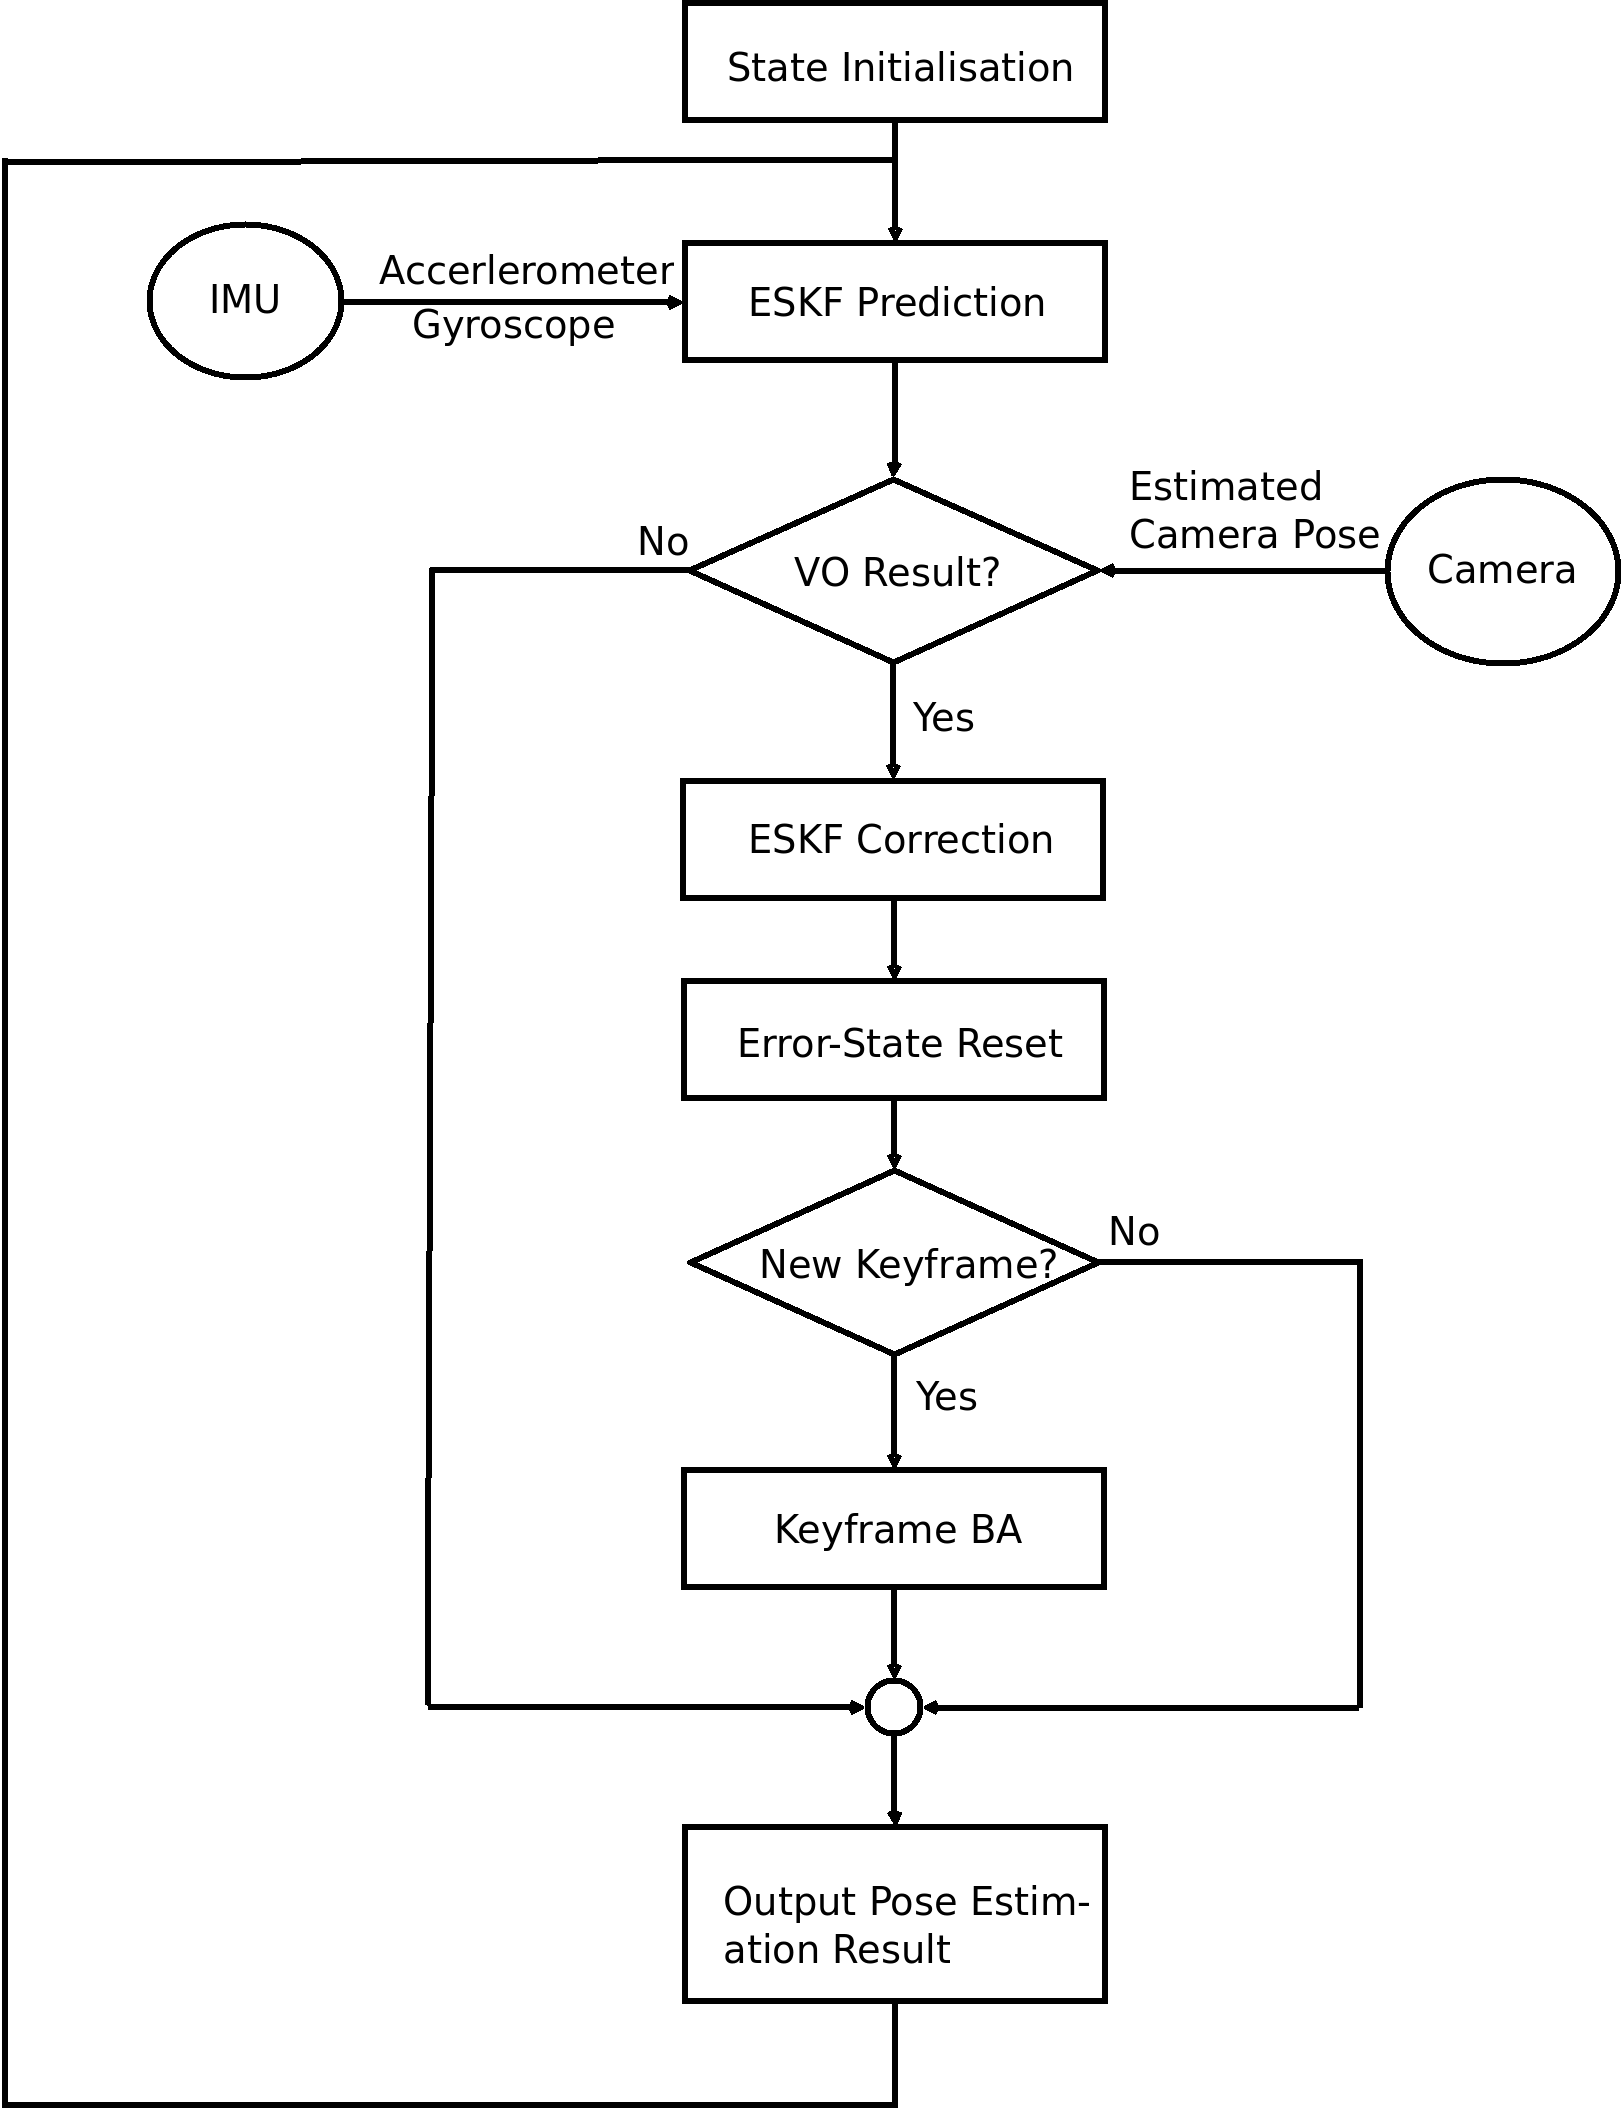
\includegraphics[width=0.5\textwidth]{CONTENT/Figure/Figure4-1_Pipeline.png}
    \caption{Pipeline of our visual-inertial odometry. Noted that measurement frequency from camera is 4 times lower than measurement frequency of IMU sensor in our experiment setting, therefore we do not have visual odometry (VO) result in some certain turn. Also whether this frame is keyframe is provided by VO.}
    \label{fig:fig4-1}
\end{figure}


In this section we summarize our visual-inertial odometry pipeline (see Figure \ref{fig:fig4-1}). We also analyses the computational cost of our visual inertial odometry system in this section.

An initialisation step is necessary for both nominal state and error state. After the system obtains measurements (\eg, 3-vector from accelerometer, and 3-vector from gyroscope) from IMU sensor, nominal state and error state are then predicted using Equation (\ref{f12}) to (\ref{f8}), and the system updates corresponding covariance matrix using Equation (\ref{f30}). 

If camera gives estimated camera pose in this turn, the system applies a \textit{correction step} as we have described in Section \ref{subsec:ESKF_IMU_sub4}. After injecting error state from nominal state, we obtain the estimated true state which contains camera pose. System then reset the error state, and further improving the odometry estimation quality by applying a keyframe bundle adjustment (keyframe BA) if this camera frame is specified as key frame by visual odometry as we have discussed in Section \ref{subsec:camera_comple_data_sub3}. Finally system output the estimated camera pose and starts the next round after receiving IMU measurements.

In our ESKF framework, computational complexity remains constant since we only keep the current states and covariance, and the size of states and covariance matrix are fixed during estimation process. To certify, we design an experiment (see Section \ref{subsec:experiment1}) to show that computational time remains unchanged when running a single IMU integration process using ESKF. As we discuss in Section \ref{sec:FVK}, the computational complexity is 
\begin{equation}
	O(m^2 \cdot n),
\end{equation}
where $m$ is the number of key frame, and $n$ is the number of landmarks. We claim that our odometry can also be extended to large scale since the number of landmarks can be enlarged and this in general is the key factor of limiting the scalability of SLAM-like system. Moreover it is also more beneficial to obtain high estimation accuracy by increasing the number of landmarks than number of key frames \cite{strasdat2010real}.

We are not able to build a environment map due to the time limitation of this master thesis. Although a few more map optimization steps are needed, the key frame BA we propose in Section \ref{subsec:camera_comple_data_sub3} gives a direct result of optimized landmarks, which are the main components of mapping. We explore this in future work chapter (Chapter \ref{chap:summary}).

All together, in this chapter we suggest an error-state Kalman filter (ESKF) based visual-inertial odometry. The system accurately estimates the camera-IMU platform pose by fusing the measurements from IMU and camera sensors. By using a loosely-coupled approach, system runs ESKF in a constant computational complexity and needs no special initialization steps, therefore it is suitable for localization of mobile robot in real-time. This odometry can also be extended to the large scaled scene, and/or an efficient SLAM system.


%% This is an example first chapter.  You should put chapter/appendix that you
%% write into a separate file, and add a line \include{yourfilename} to
%% main.tex, where `yourfilename.tex' is the name of the chapter/appendix file.
%% You can process specific files by typing their names in at the 
%% \files=
%% prompt when you run the file main.tex through LaTeX.
\chapter{Experiments}
\label{chap:experiments}

% % remove all spaces between columns in tables
% \setlength{\tabcolsep}{0.3pt}
% % remove all spaces below captions
% \setlength{\belowcaptionskip}{-5pt}

\section{Synthetic Dataset}
\label{sec:sync_data}

\section{Some other experiments}

% 
\chapter{Discussion}

%% This is an example first chapter.  You should put chapter/appendix that you
%% write into a separate file, and add a line \include{yourfilename} to
%% main.tex, where `yourfilename.tex' is the name of the chapter/appendix file.
%% You can process specific files by typing their names in at the 
%% \files=
%% prompt when you run the file main.tex through LaTeX.
\chapter{Summary, Discussion and Future Works}
\label{chap:summary}

%In conclusion, we suggest a robust sensory fusing framework to be applied on visual-inertial odometry. This framework is lead by integrating IMU measurement from local frame to global frame, with additional extrasensory data (vision data) to complement unobservable parameters of IMU. We further explore a self-adapt map scale method and keyframe-based local bundle adjustment to increase the estimation accuracy.

%The advantages of this framework is that system does not keep visual landmarks and IMU measurement, therefore runs in a constant time complexity, which can be easily extended a large scaled scene. The drawback is that it is more reliable to the performance of visual odometry, meaning that if the correction data gives bad feedback, the whole system is easily collapsed. However we have provided experimental results that our framework can give more stable and accuracy estimation of camera pose than current state-of-art visual odometry on same data sequence, thus we argue that our work is meaningful and the results of our system will further be increased with the development of visual odometry.

%Another way to resolve this drawback is to apply feature-based visual-inertial methods (tightly-coupled IMU integration), which could be a potential future work. More recent literatures show that feature-based VIO performs well and can be used commercially. \cite{forster2015imu} uses pre-integration theory and manifold optimization to optimize IMU and visual information together; \cite{hesch2014consistency}, which is considered the foundation algorithm of Google Project Tango, runs a consistency analysis and modify some terms of traditional IMU integration to obtain less variation results. Unfortunately, we could not compare those latest algorithm due the un-release of their codes, it is definitely worth to try their ideas of VIO in the future. Though in such tighly-coupled visual-inertial SLAM, computational complexity is severely increased, therefore more simplifications of optimization step has to be explored, like pre-integration theory applied in \cite{forster2015imu}. 

%Due to the lack of resources and time, we are not available to build a real IMU-camera platform in this master thesis. A more rigorous denoise technique and more complicated noise model might have to be applied when using real data, which is also a possible way to work with in the future. 

In this master thesis, we have suggested a robust sensory fusing framework, which can be applied on real-time mobile robot navigation. Visual data (\eg, images) can provide adequate information, however it is rather time-consuming to analysis; while the inertial sensor (IMU) provides accurate estimation of its observable variables but needs compensation in its unobservable parameters. We aim to improve the localization quality by fusing such multiple sensory data. This framework is lead by integrating IMU measurement from local frame to global frame, with additional extrasensory data (vision data) to complement unobservable parameters of IMU. We further explore a self-adapt map scale method and keyframe-based local bundle adjustment to increase the estimation accuracy.

In experimental parts, we demonstrate several experiments to provide evidences that our framework is robust and correct. First we examine our IMU integration method in regular and special trajectory independently, second we show that our framework is more robust and accurate than single visual odometry, at last we show that a keyframe-based local bundle adjustment to further increase the estimation accuracy, and whole system runs in real-time.

The advantages of this framework is that system does not need to keep visual landmarks and IMU measurement, therefore runs in a constant time complexity. Moreover it can be easily extended a large scaled scene. The drawback is that such a framework can be regarded as a single iteration of optimization step, hence the solution is sub-optimal. As we have discussed in the first few parts, the trade-off of computational complexity and estimation accuracy is inevitable, once we have used complete optimization solution, system will keep certain numbers of former states, hence it might be more time-consuming.

We briefly introduce our current interests in Chapter \ref{chap:current}. We are supposed to show that our ESKF IMU integration framework can be transformed into a non-linear optimization solution easily. The cost function is formed by visual error (reprojection error) and IMU temporal error. By establishing such a cost function, one can solve it by performing a manifold optimization methods as we have introduced in Section \ref{sec:exponential}. One thing left is to decrease the computational time in optimization step, such as landmark position elimination (structureless approach) in tightly-coupled VIO \cite{mourikis2007multi, forster2015imu}, or pre-integration theory \cite{forster2015imu} to avoid repeatedly computing IMU integration. Another potential improvement is based on the work in \cite{hesch2014consistency}, which provides a consistency analysis and modify some terms of traditional IMU integration formulations, and eventually obtain estimation results with less variations.

We are not able to build a real IMU-camera platform in this master thesis due to the lack of resources and time. A more rigorous denoise technique and more complicated noise model might have to be applied when using real data, which is also a possible working area in the future.


\appendix
\chapter{The Derivation of Error-state Kinematic Equations}
\label{chap:appendix1}

We here derive Equation (\ref{f4}) and Equation (\ref{f5}) in Chapter \ref{chap:sensor_fusing}.

In order to simplify our notation, we define
\begin{align}
	\label{a1}
	\vec{a}_n &\triangleq \vec{a}_m - \vec{a}_{bn} \\
	\label{a2}
	\vec{\omega}_n &\triangleq \vec{\omega}_m - \vec{\omega}_{bn} \\
	\label{a3}
	\vec{a}_e &\triangleq -\vec{a}_{be} - \vec{a}_n \\
	\label{a4}
	\vec{\omega}_e &\triangleq -\vec{\omega}_{be} - \vec{\omega}_n 
\end{align}

We derive Equation (\ref{f4}) by
\begin{align}
	\dot{\vec{v}}_e &= \dot{\vec{v}}_t - \dot{\vec{v}}_n \\
			  &= (\mR_t\vec{a}_t +\vec{g}_t) - (\mR_n\vec{a}_n +\vec{g}_n)
\end{align}
we then uses small signal approximation for $R_t$ by Equation (\ref{q25}) and Equation (\ref{q30}), which leads to 
\begin{equation}
	\mR_t = \mR_n(\ones + \left[ \vec{\theta}_n \right]_\times) + O(\norm{\Delta{\vec{\theta}_e}}^2)
\end{equation}
we omit the second order of angular term and followed by Equation (\ref{f11}), we obtain
\begin{align}
	\dot{\vec{v}}_e &= (\mR_n(\ones + \left[ \vec{\theta}_n \right]_\times)\vec{a}_t +\vec{g}_t) - (\mR_n\vec{a}_n +\vec{g}_n) \\
					&= \mR_n(\ones + \left[ \vec{\theta}_n \right]_\times)(\vec{a}_n+\vec{a}_e)+\vec{g}_e
\end{align}
By applying the property of skew-symmetric matrix $\left[ \vec{a} \right]_\times \vec{b} = \left[ \vec{b} \right]_\times \vec{a}$, and recalling (\ref{a1}), (\ref{a2}). We have
\begin{align}
	\dot{\vec{v}}_e &= \mR_n \left[ \vec{a}_m - \vec{a}_{bn} \right]_{\times} -  \mR_n\vec{a}_{be} + \vec{g}_e - \mR_n\vec{a}_n
\end{align}
which is exactly Equation (\ref{f4}).

We then derive Equation (\ref{f5}) by 
\begin{align}
	\dot{\vec{q}}_e &= \frac{1}{2}(\vec{q}_e \otimes \vec{\omega}_t - \vec{\omega}_n \otimes \vec{q}_e)
\end{align}
and we have pure quaternion $\dot{\vec{\theta}}_e = 2\dot{\vec{q}}_e$. By expanding all terms in above equations, we have
\begin{align}
	\dot{\vec{\theta}_e} &= -\left[ \vec{\omega}_n \right]_\times\vec{\theta}_e + \vec{\omega}_e + O(\norm{\Delta{\vec{\theta}_e}}^2)
\end{align}

By omitting all second-oder terms and recalling (\ref{a3}), (\ref{a4}), we obtain
\begin{align}
	\dot{\vec{\theta}_e} =& \left[ \vec{\omega}_m - \vec{\omega}_{bn} \right]_{\times} - \vec{\omega}_{be} - \vec{\omega}_{n}
\end{align}
which is Equation (\ref{f5}).
\chapter{Integration Methods}
\label{chap:appendix2}

\section{Runge-Kutta Numerical Integration Methods}
\label{sec:runge_kutta}

Runge-Kutta methods aims to give a approximate solutions of ordinary differential equations, \eg, our time-derivative state $\dot{\vec{x}}$, which is 
\begin{equation}
	\dot{\vec{x}} = f(t, \vec{x})
\end{equation}
The solution give in Equation (\ref{f12}) - (\ref{f13}) by simplest version of Runge-Kutta methods, \eg, assuming $\dot{\vec{x}}$ over each time period $\Delta{t}$, which gives us
\begin{equation}
	\vec{x}_{n+1} = \vec{x}_{n} + f(t_n, \vec{x}_n)\Delta{t}
\end{equation}
More complicated Runge-Kutta methods please refers to \cite{wiki:RK4}.

\section{Closed-form Integration Methods}
\label{sec:close_integration}
We first gives a clean version of Equation (\ref{f5}), which is
\begin{equation}
	\dot{\vec{\theta}_e} = -\left[ \vec{\omega} \right]_\times\vec{\theta}_e
\end{equation}
we update $\vec{\theta}_e$ by
\begin{align}
	\vec{\theta}_e^{\prime} &= \vec{\theta}_e + \dot{\vec{\theta}_e}\Delta{t} \\
							\label{b1}
							&= \vec{\theta}_e -\left[ \vec{\omega} \right]_\times\vec{\theta}_e\Delta{t} \\
							\label{b2}
							&= \mR\{ -\vec{\omega}\Delta{t} \} \\
							&= \mR\{ \vec{\omega}\Delta{t} \}^T
\end{align}
which we apply Equation (\ref{q25}) and Equation (\ref{q30}) from Equation (\ref{b1}) to (\ref{b2}). This integration is a closed-form integration.
\clearpage
\newpage

\chapter{Approximation Methods}
\label{chap:appendix2}

~\cite{mourikis2007multi}

\clearpage
\newpage

%% This defines the bibliography file (main.bib) and the bibliography style.
%% If you want to create a bibliography file by hand, change the contents of
%% this file to a `thebibliography' environment.  For more information 
%% see section 4.3 of the LaTeX manual.
\begin{singlespace}
    \bibliography{BIB/mybiblio}
    \bibliographystyle{plain}
\end{singlespace}


\end{document}

